% !TeX root = ../main.tex
\section{Results}

\subsection{Model Diagnostic Performance}

\subsubsection{Sensitivity}
\begin{figure}[H]
  \centering
  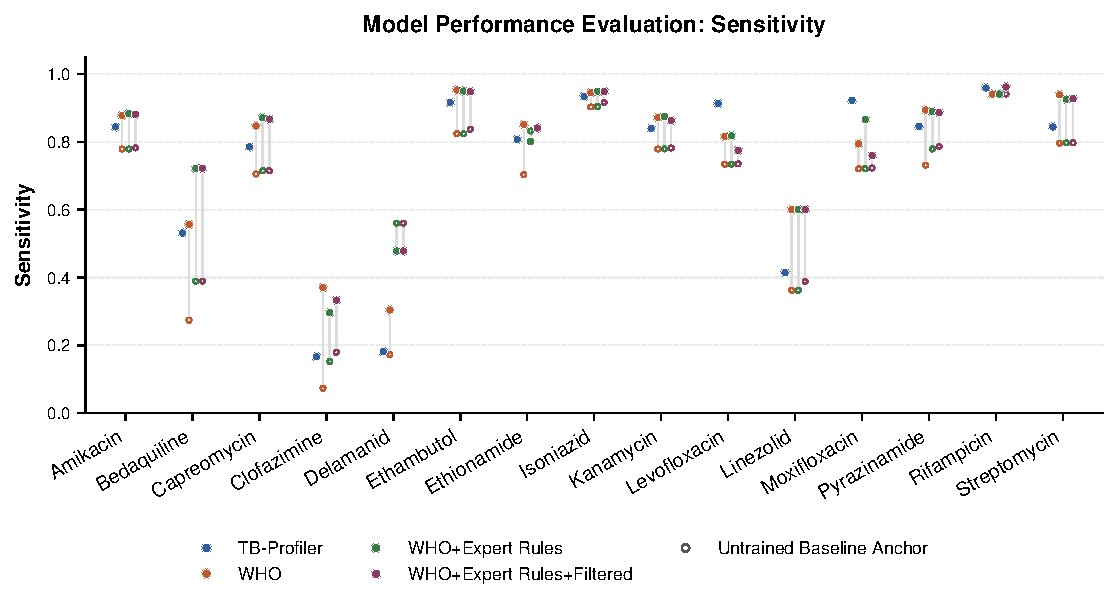
\includegraphics[width=\textwidth]{figures/sensitivity.pdf}
  \caption{Sensitivity of the neural network with tb-profiler as the baseline, WHO, and WHO augmented with
  expert rules, and filtered is shown aswell. The naive pass with only the catalogues encoded as 1s , or 0s
  is shown as empty circles, and the trained model results are filled in.}\label{fig:sens}
\end{figure}

\subsubsection{Specificity}
\begin{figure}[H]
  \begin{center}
    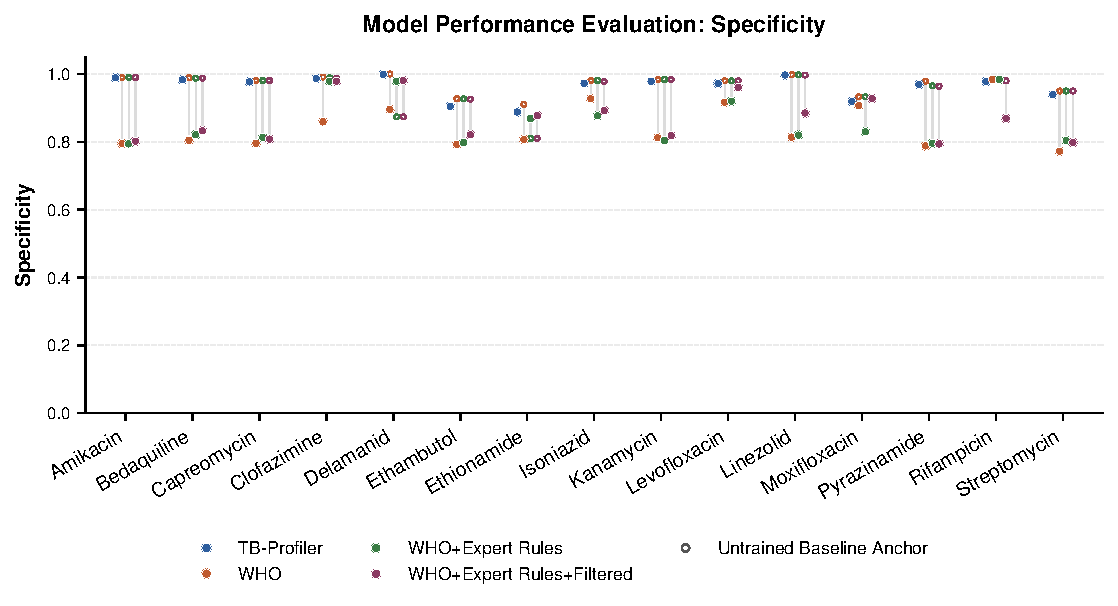
\includegraphics[width=\textwidth]{figures/specificity.pdf}
  \end{center}
  \caption{Specificity of the neural network after training for 15 Anti-TB drugs that had at final confidence
  grading of 1 or 2. TB-profiler (blue) acts as the baseline to show how the neural networks perform with different
  weights. Weights were constructed from the WHO catalogue, and then augmented with expert rules and filtered snps.
  These are represented as hollow circles, and after training, they are represented as filled circles.}\label{fig:spec}
\end{figure}

\subsubsection{F1 Score}
\begin{figure}[H]
  \begin{center}
    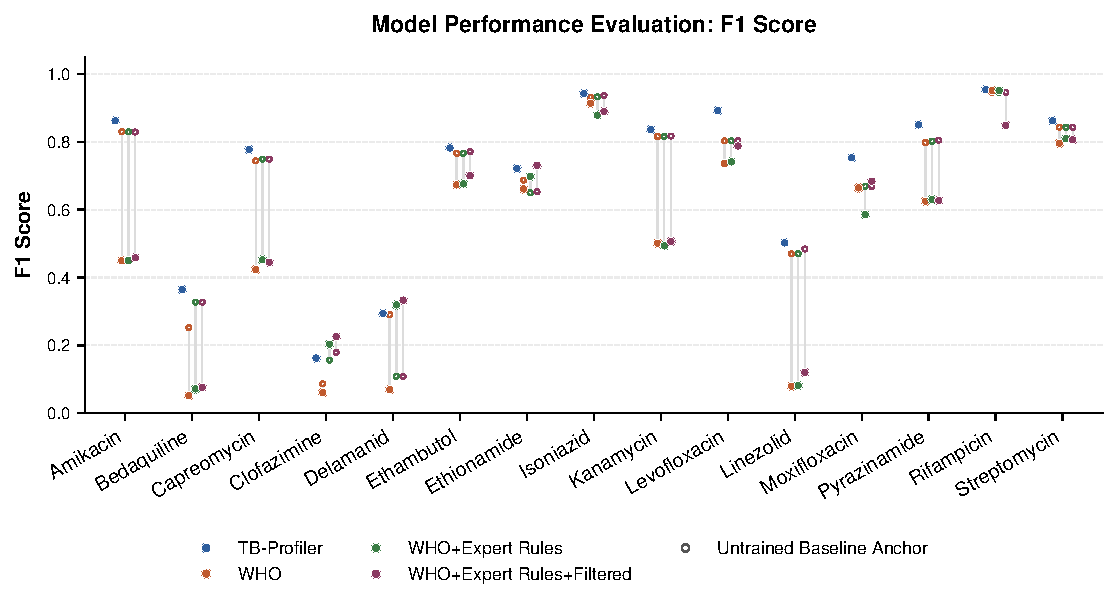
\includegraphics[width=\textwidth]{figures/f1.pdf}
  \end{center}
  \caption{F1 scores of the neural networks, with F1 being the balanced average between specificity and sensitivity.
  In this plot, TB-profiler is used as a baseline, colored in blue, and the untrained networks with shown with hollow
  circles. The trained models are shown with filled circles.}\label{fig:f1}
\end{figure}

\subsection{Classification Performance Across Weight Schemes}

\begin{figure}[H]
  \begin{center}
    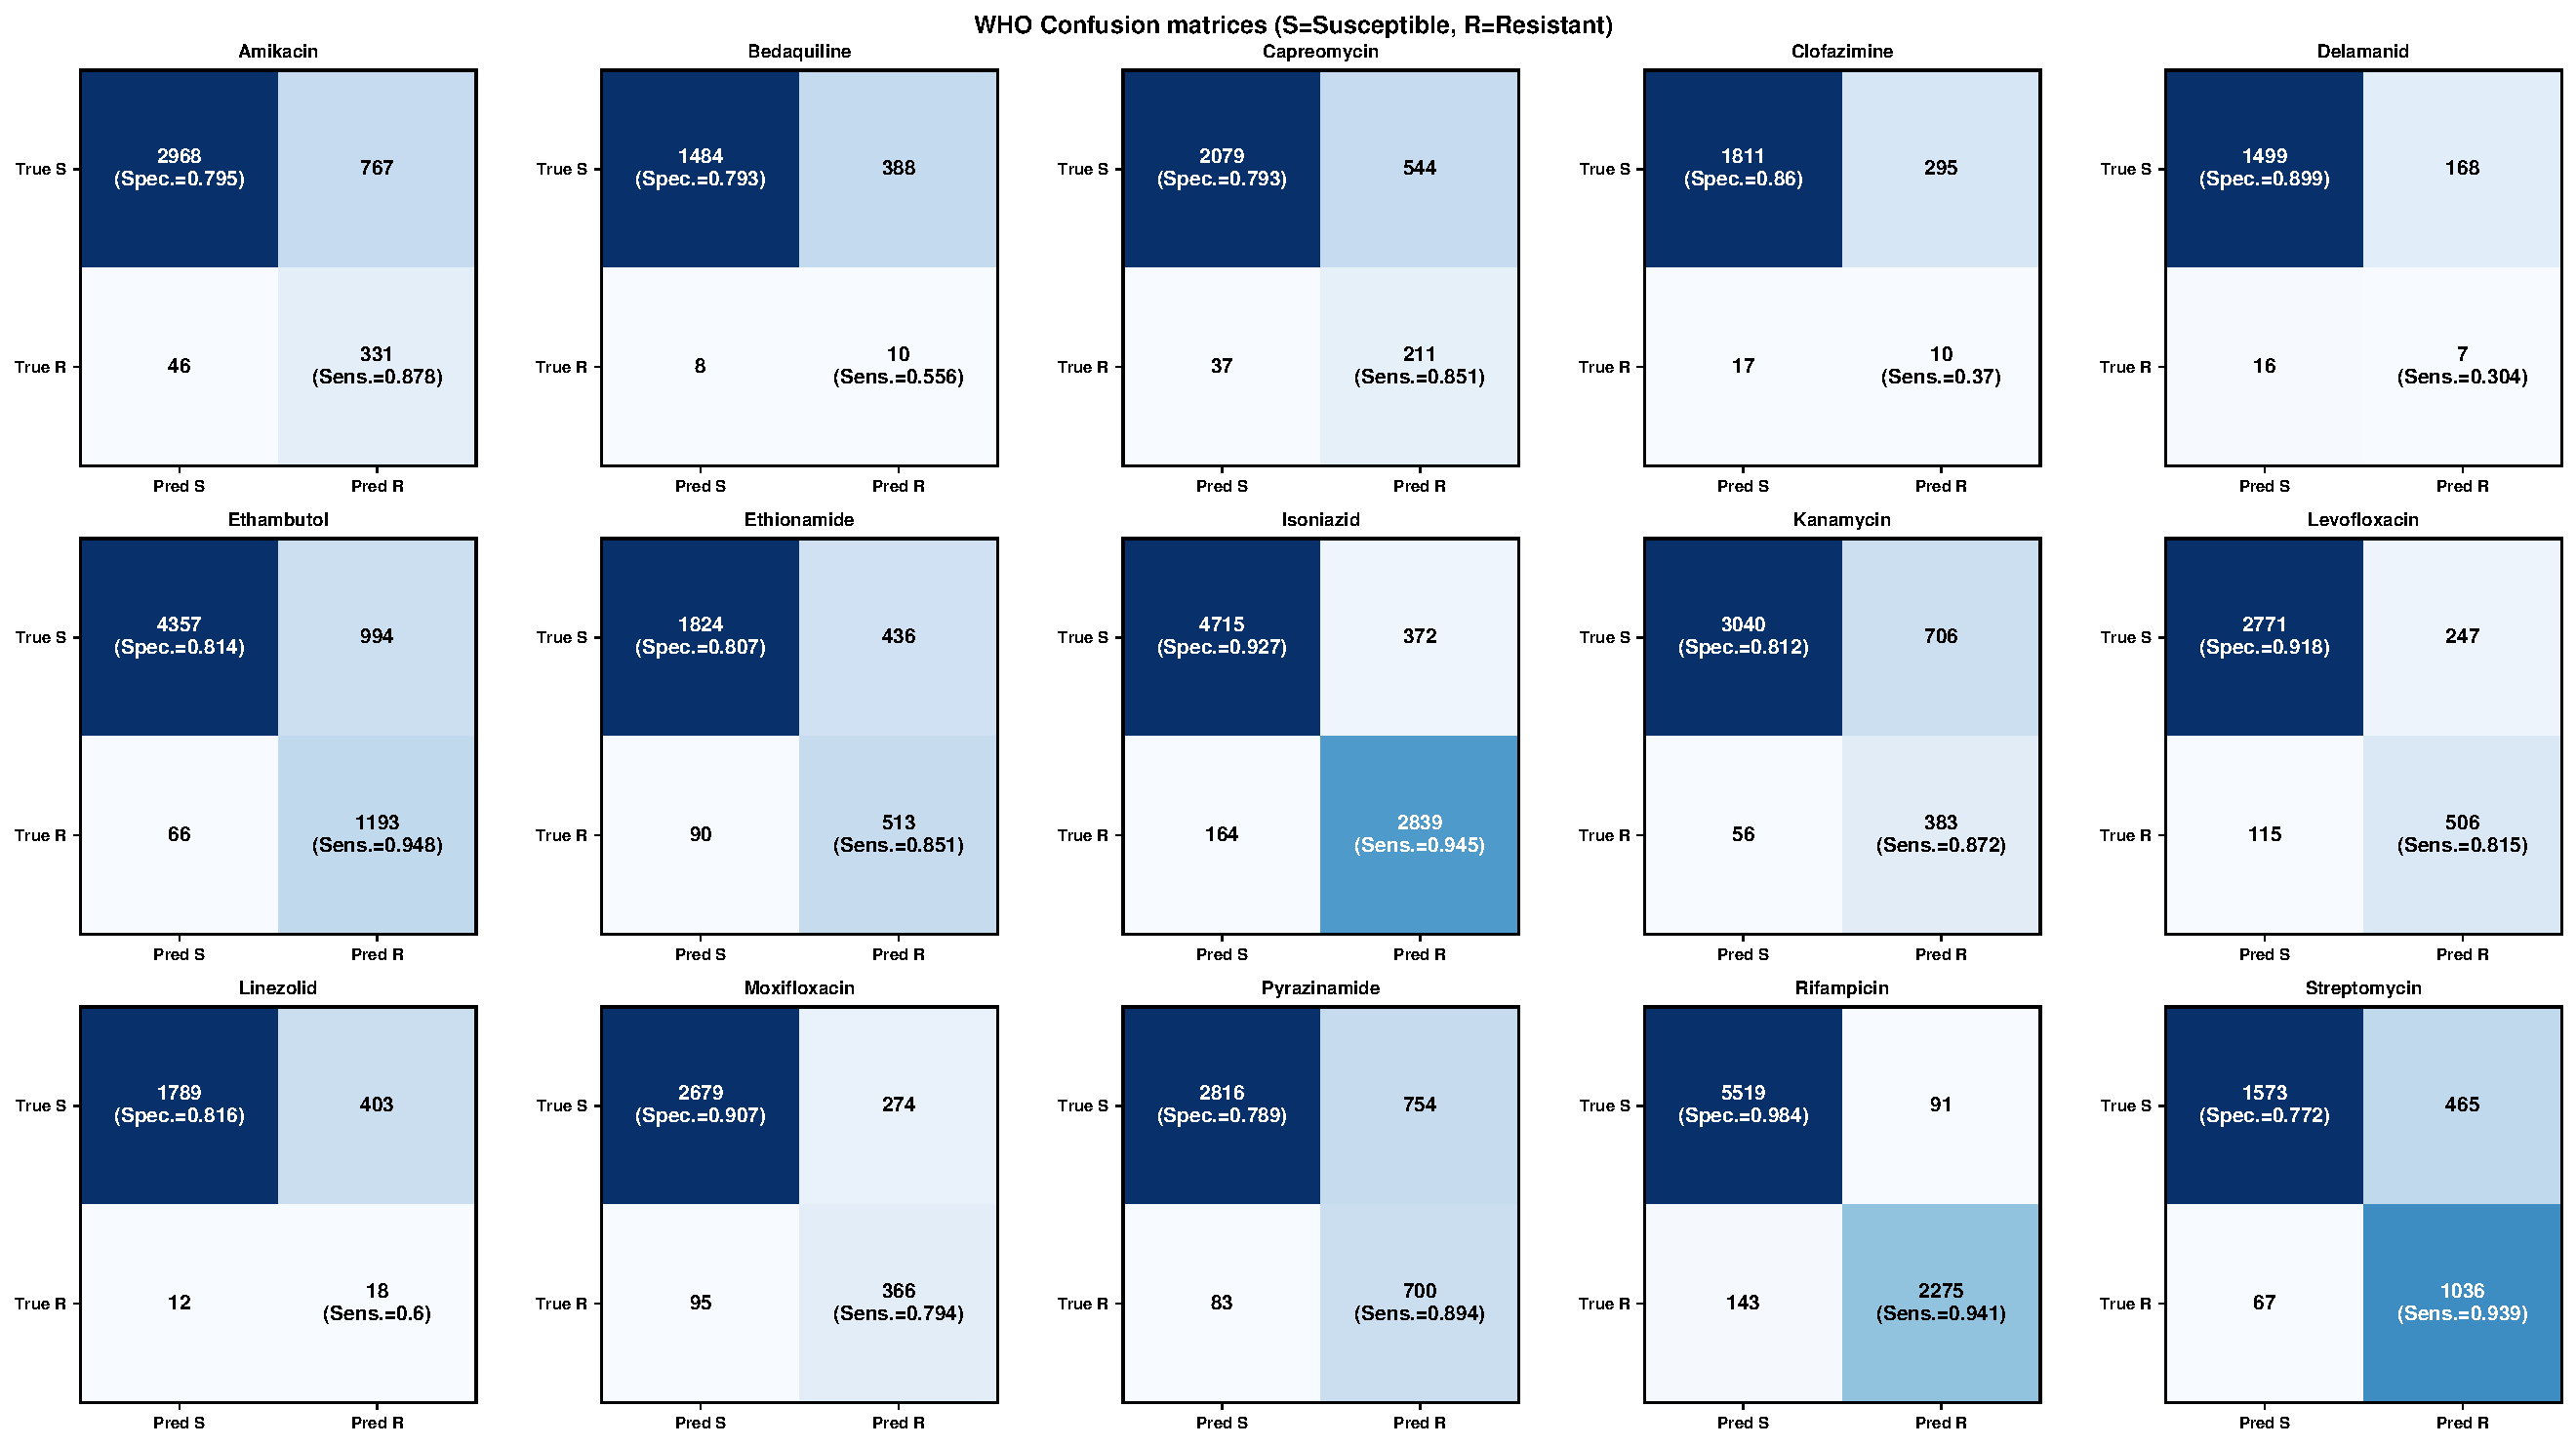
\includegraphics[width=\textwidth]{figures/who_confusion_matrices.pdf}
  \end{center}
  \caption{Confusion matrix for 15 drugs for the WHO snp catalogue}\label{fig:whocm}
\end{figure}

\begin{figure}[H]
  \begin{center}
    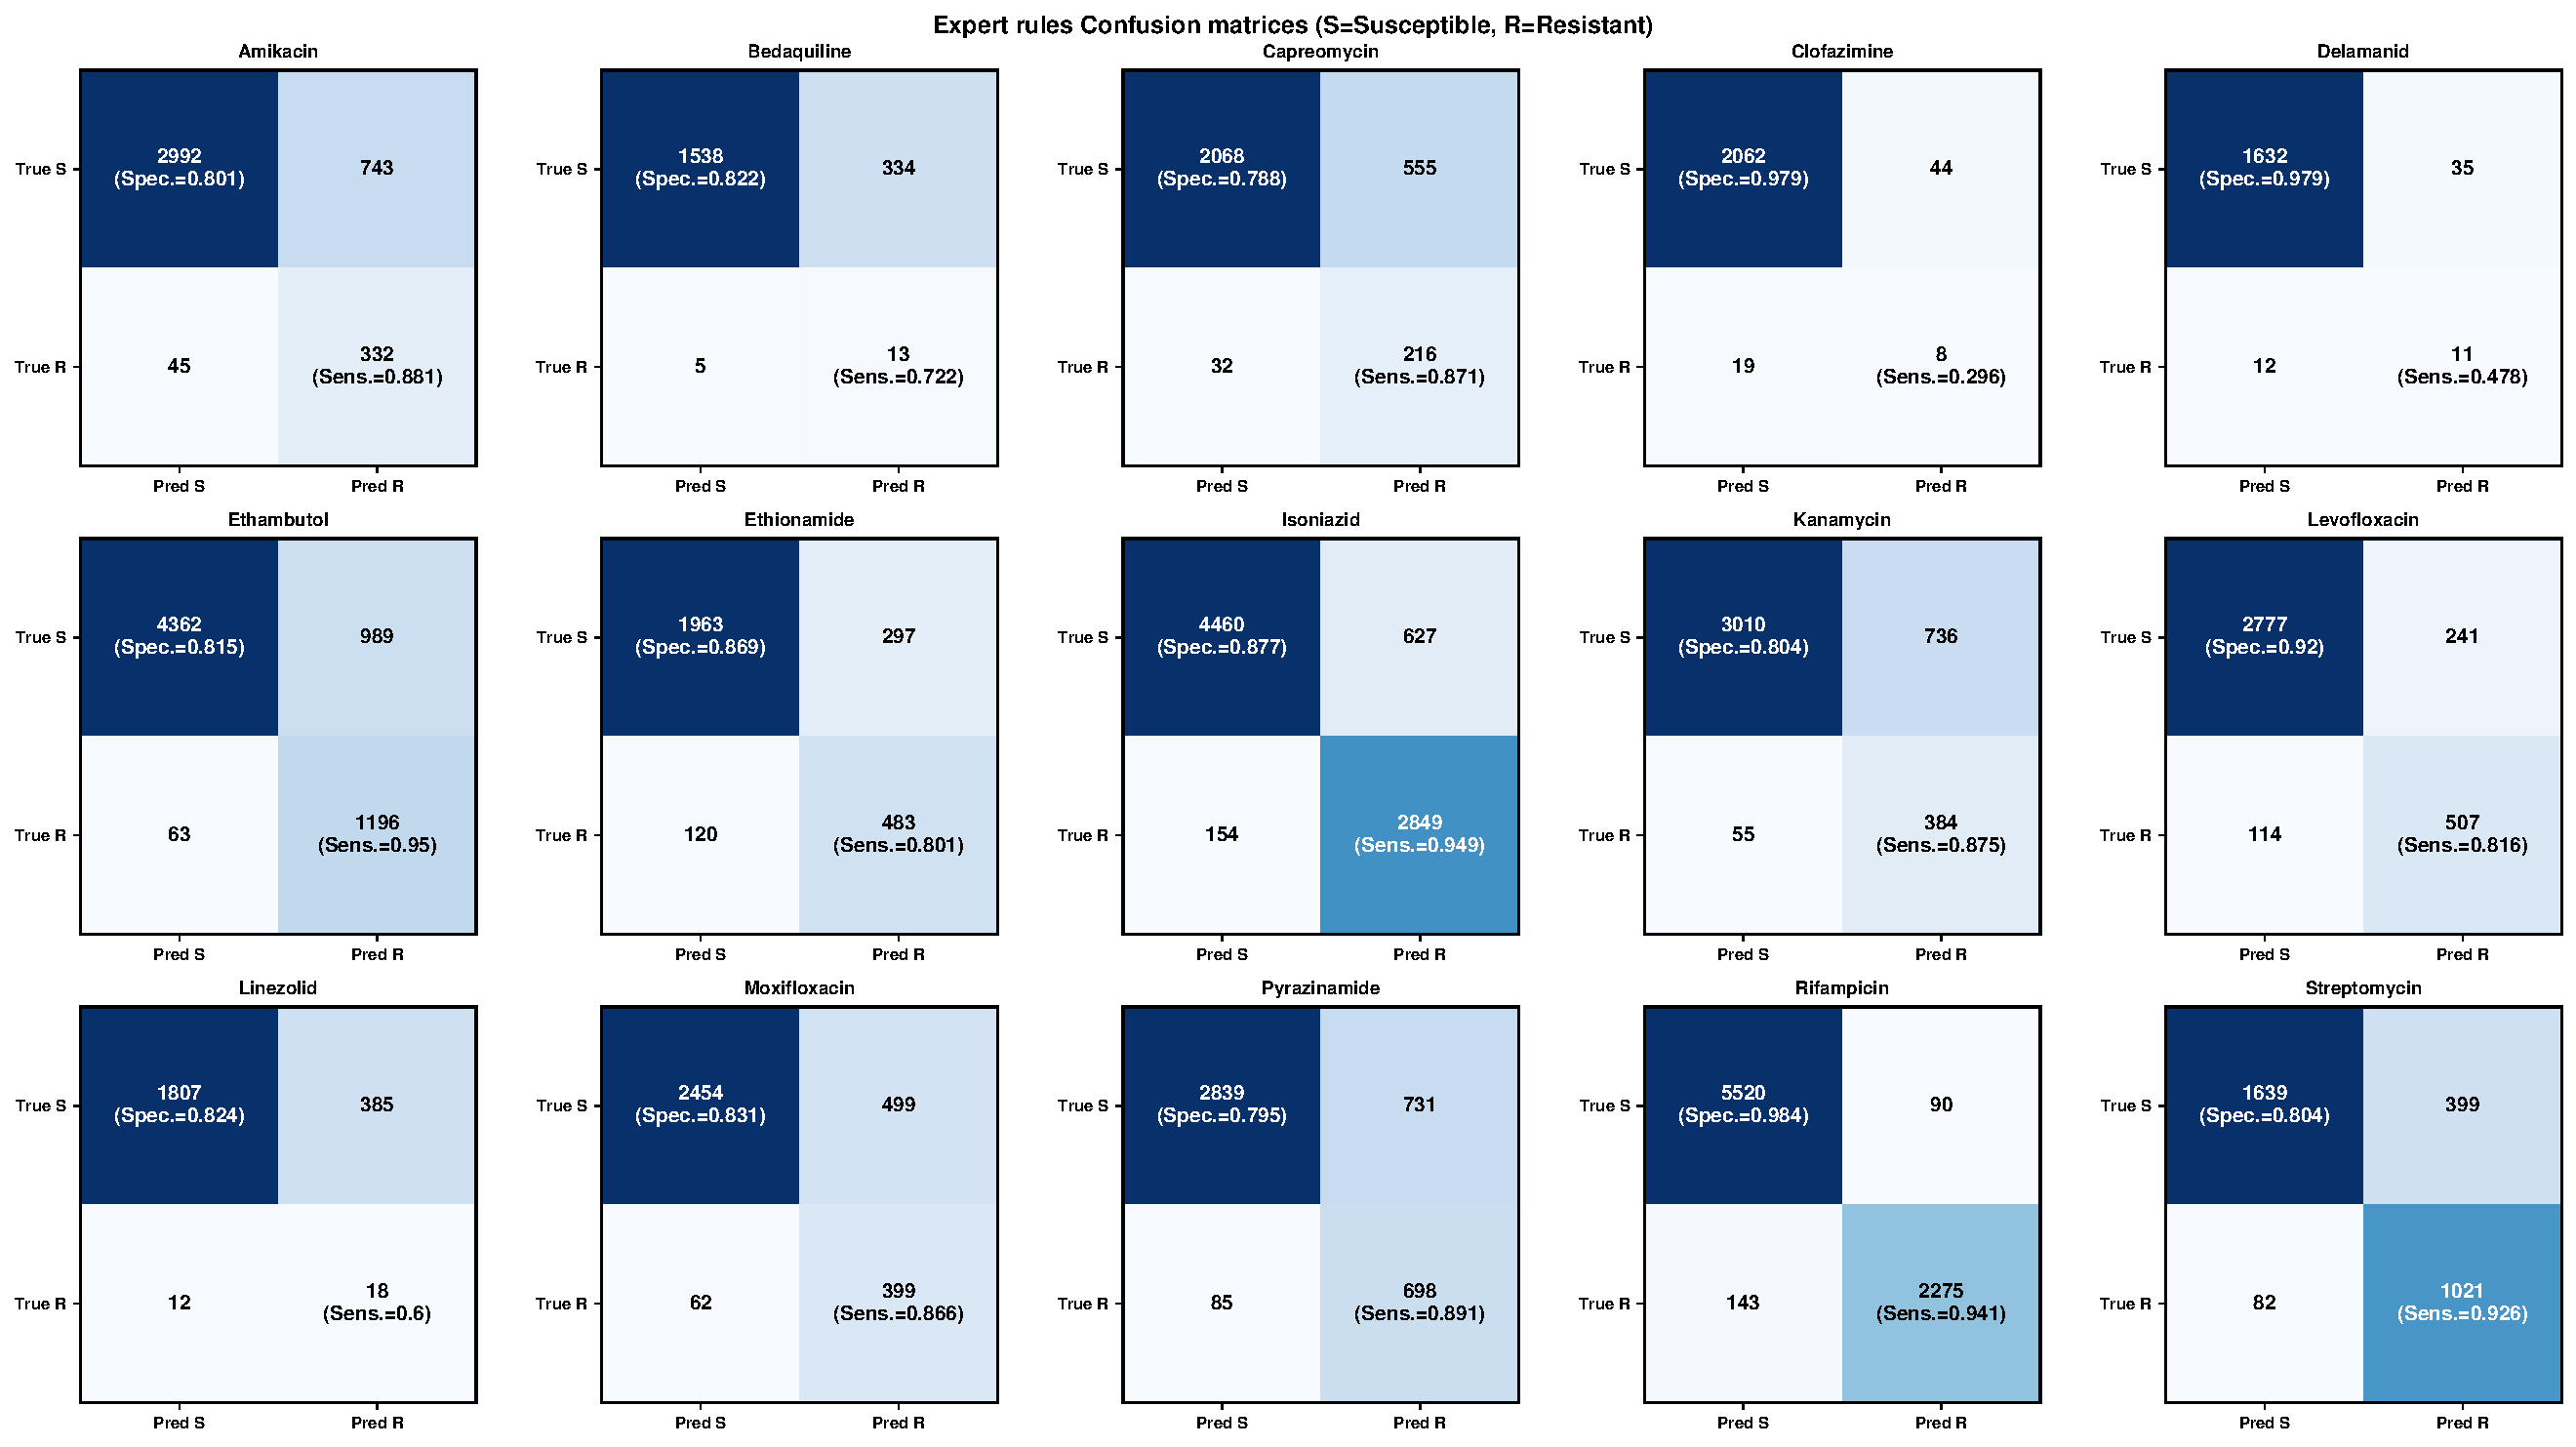
\includegraphics[width=\textwidth]{figures/expert_rules_confusion_matrices.pdf}
  \end{center}
  \caption{Confusion matrix for er+who catalogue.}\label{fig:ercm}
\end{figure}

\begin{figure}[H]
  \begin{center}
    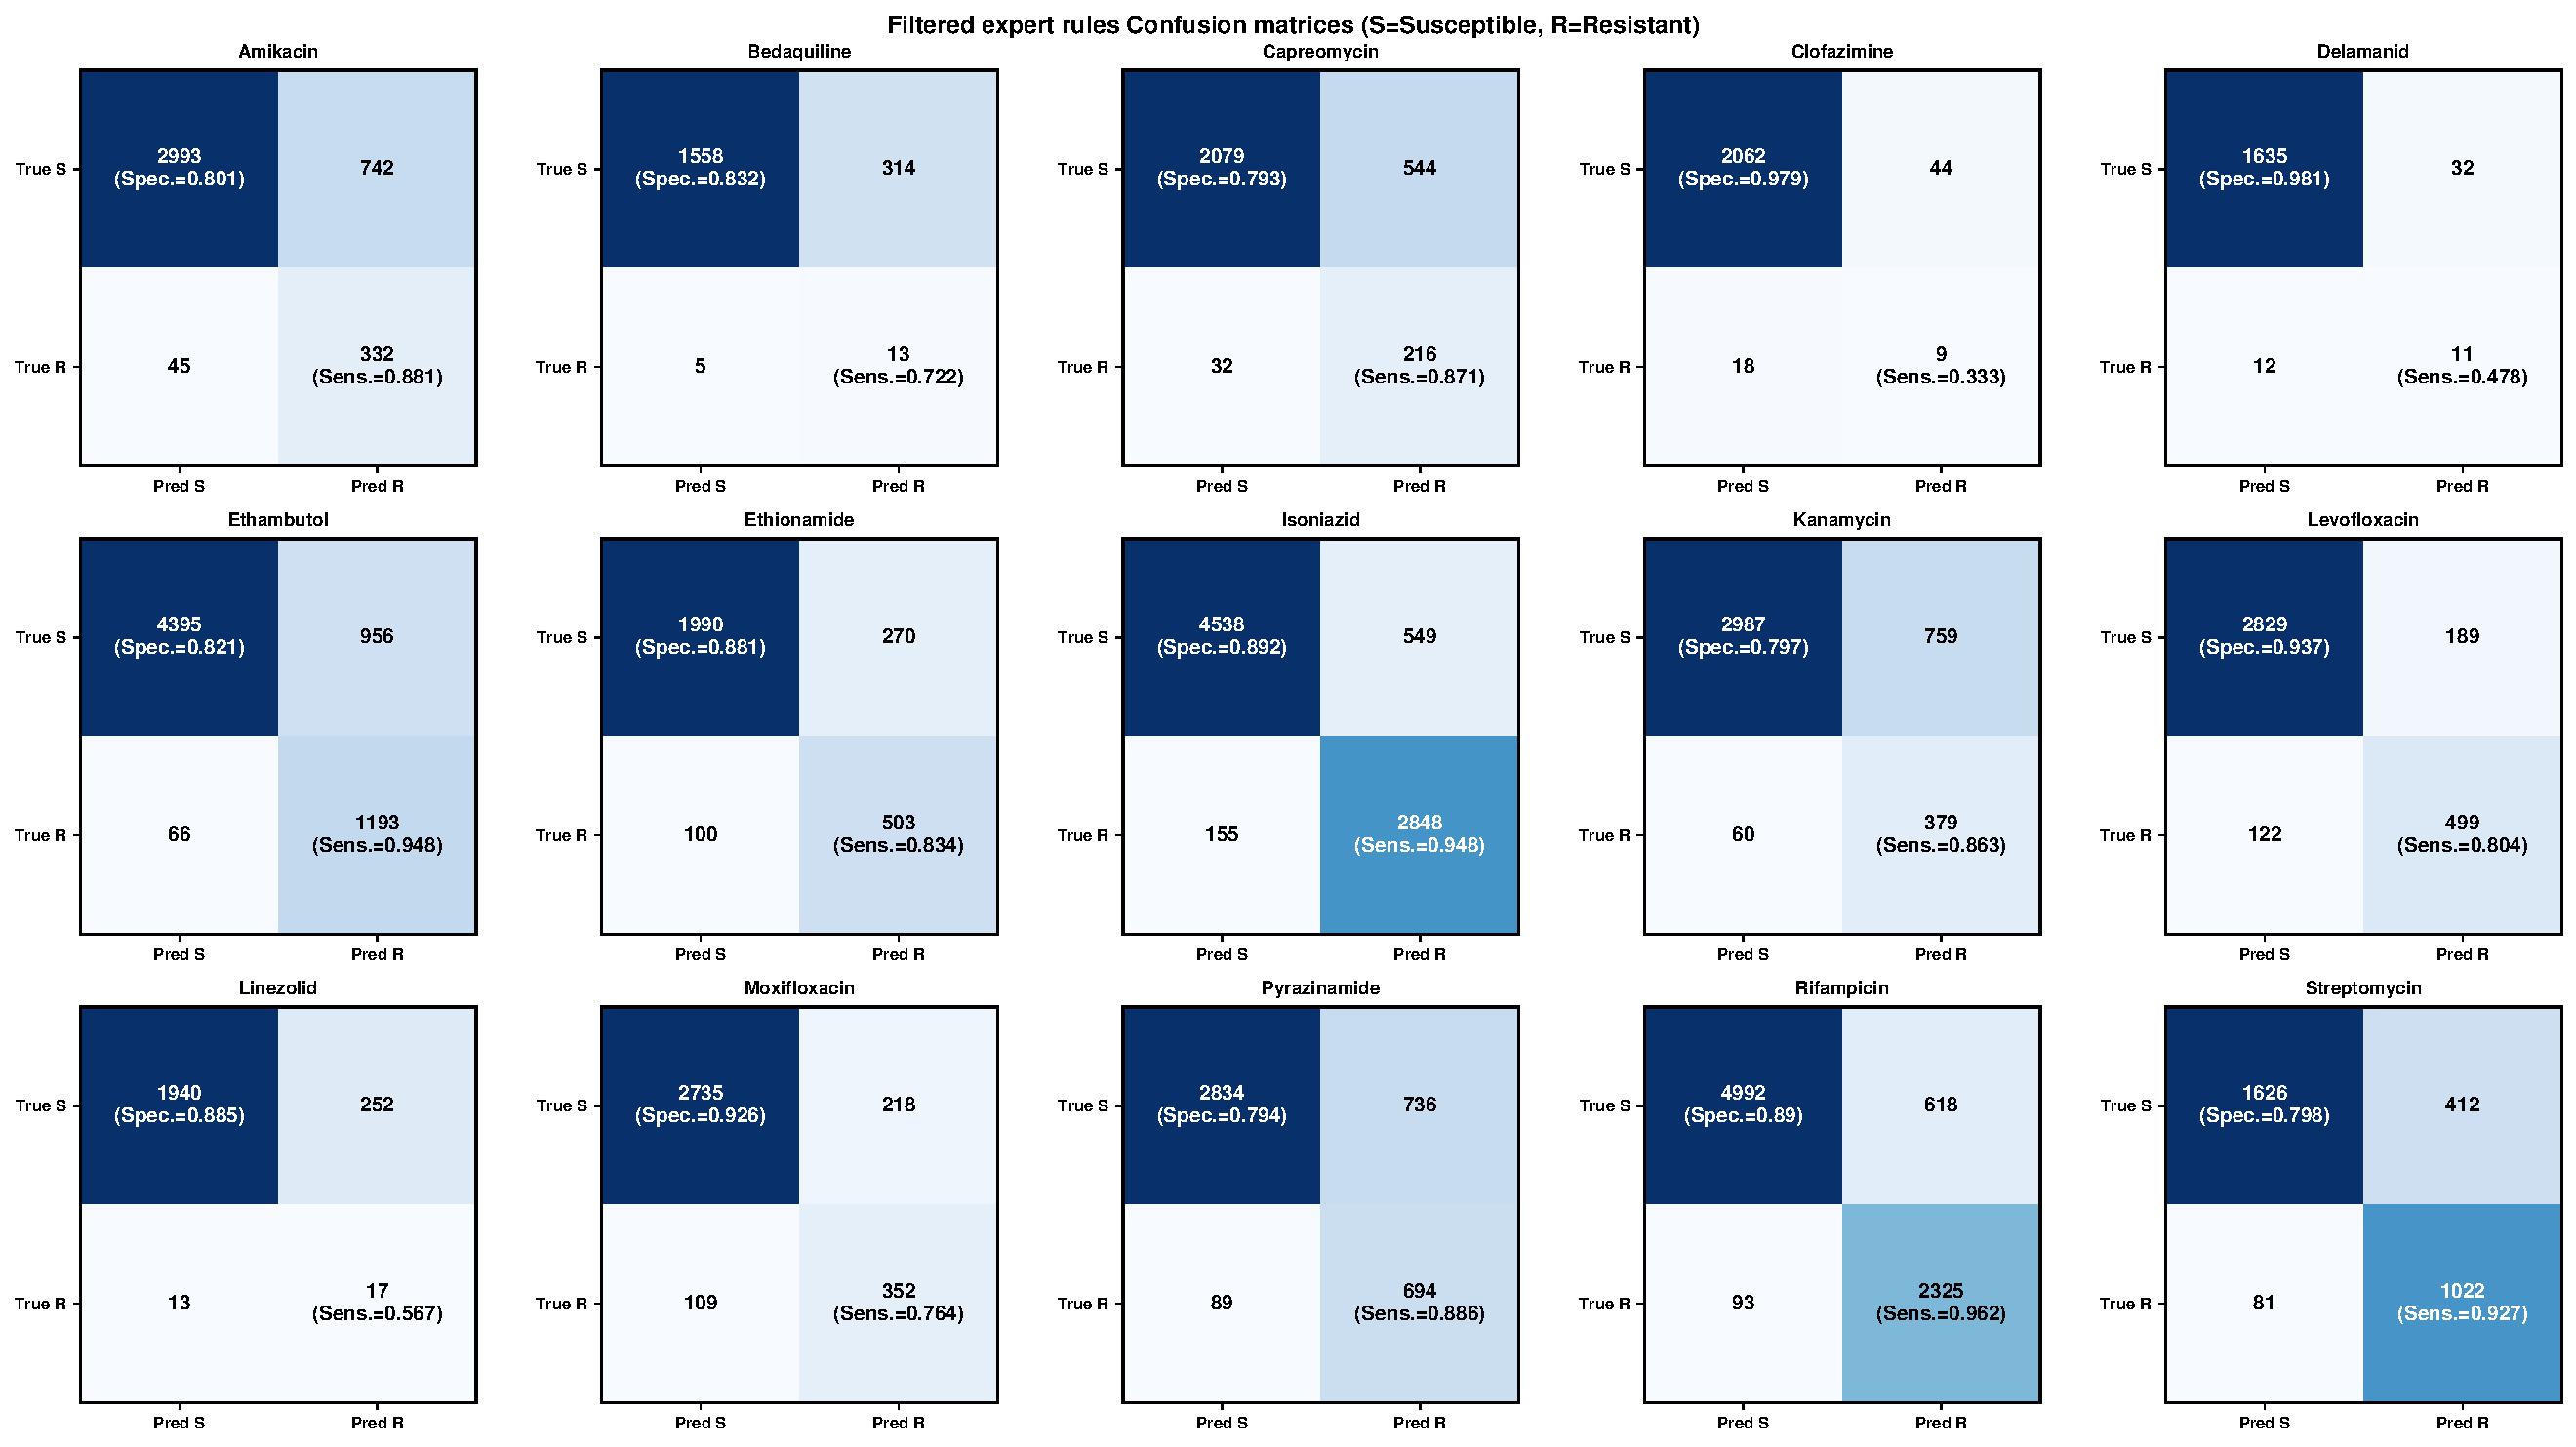
\includegraphics[width=\textwidth]{figures/filtered_expert_rules_confusion_matrices.pdf}
  \end{center}
  \caption{Confusion matrix for er+who+filt catalogue.}\label{fig:filtcm}
\end{figure}

\subsection{Training and Validation Convergence}

\begin{figure}[H]
  \begin{center}
    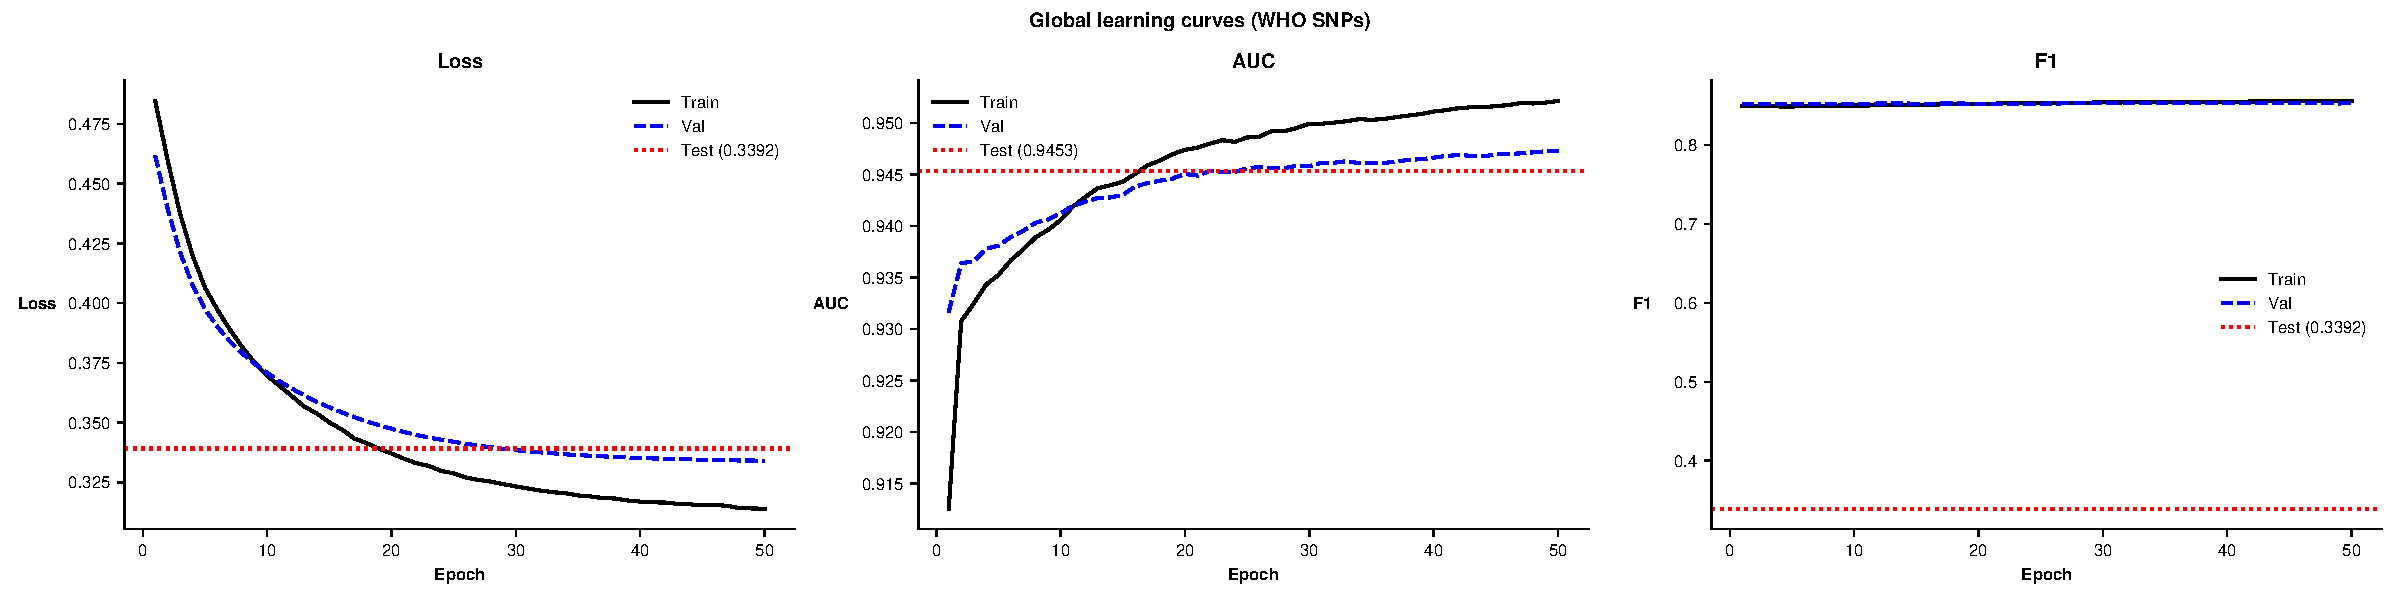
\includegraphics[width=\textwidth]{figures/who_learning_curves.pdf}
  \end{center}
  \caption{Global learning curves for who catalogue.}\label{fig:wholr}
\end{figure}

\begin{figure}[H]
  \begin{center}
    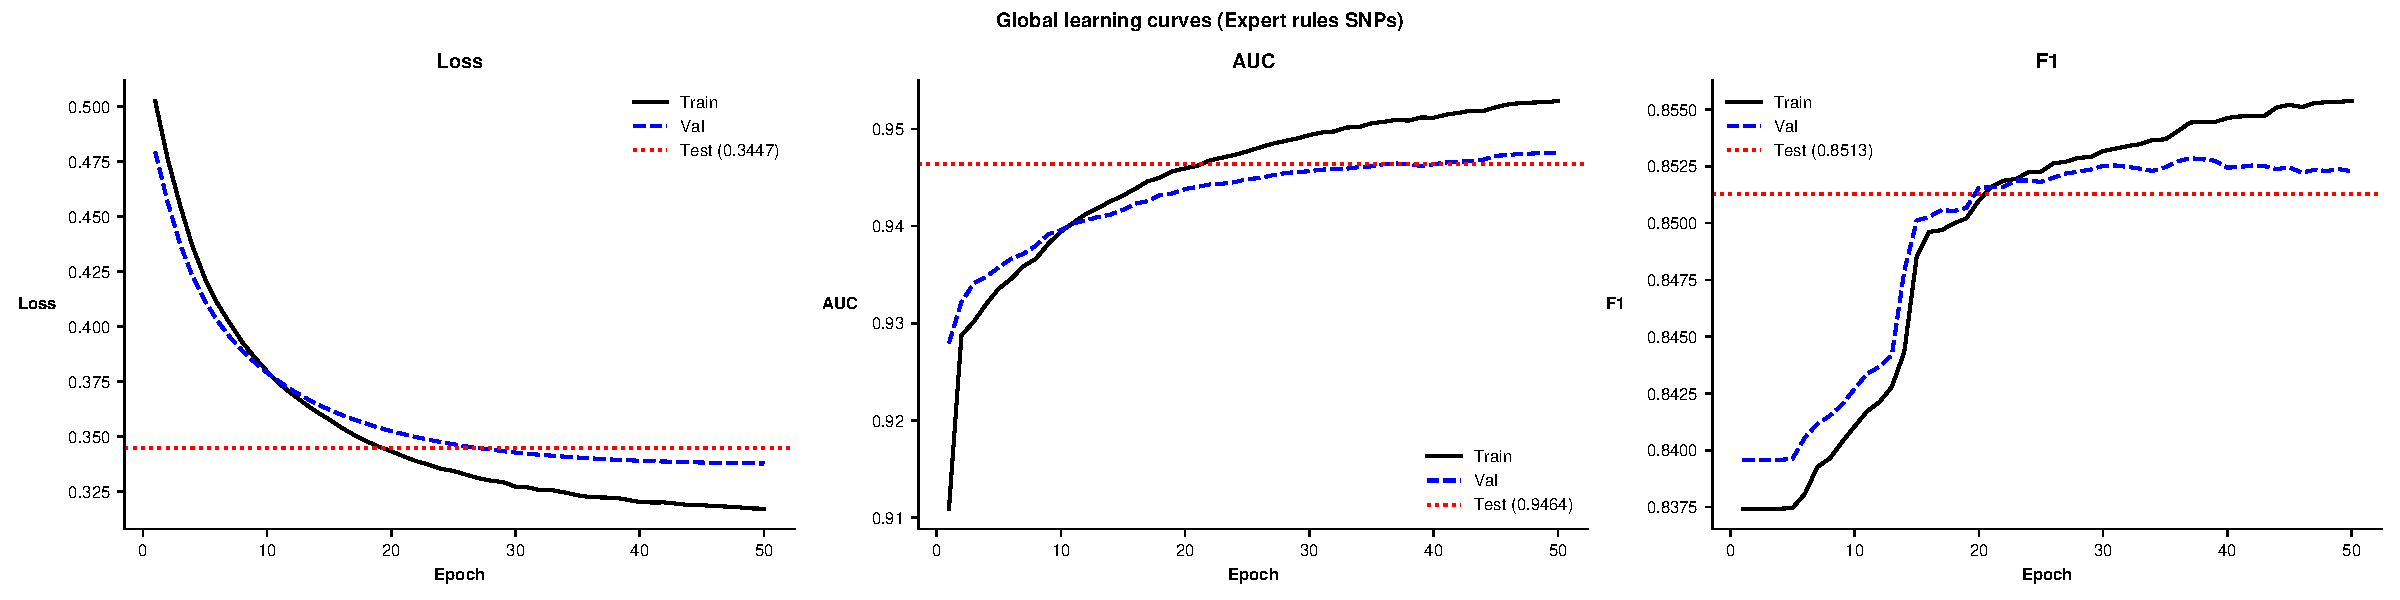
\includegraphics[width=\textwidth]{figures/expert_rules_learning_curves.pdf}
  \end{center}
  \caption{Global learning curves for er+who catalogue.}\label{fig:erlr}
\end{figure}

\begin{figure}[H]
  \begin{center}
    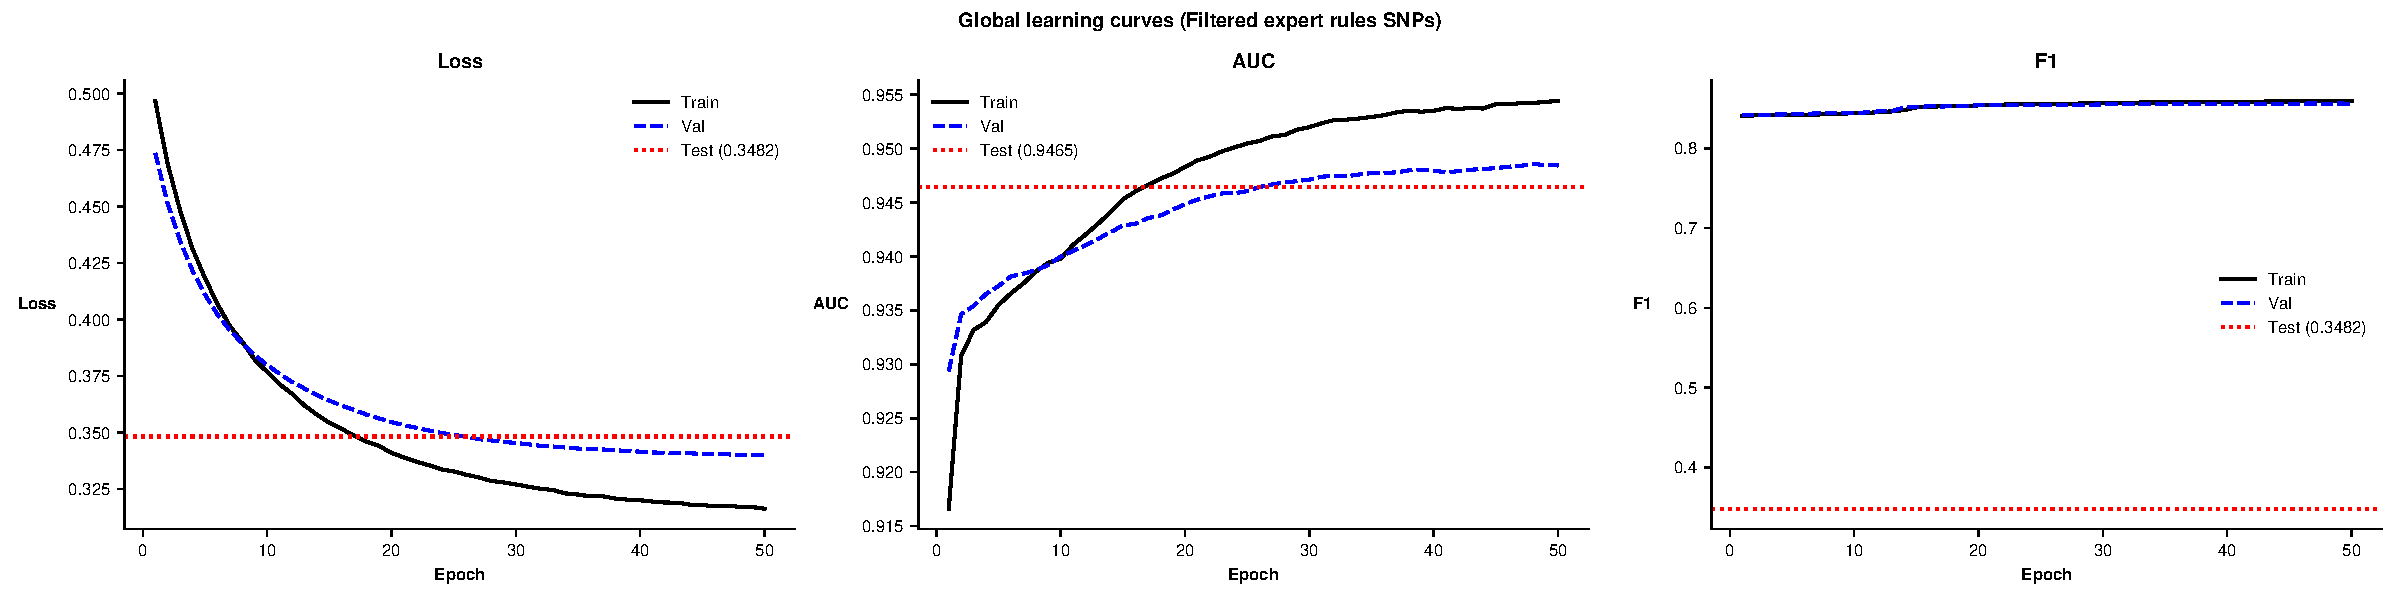
\includegraphics[width=\textwidth]{figures/filtered_expert_rules_learning_curves.pdf}
  \end{center}
  \caption{Global learning curves for er+who catalogue.}\label{fig:erlr}
\end{figure}



\subsection{Per-drug Learning Curves}
% Page 1
\begin{figure}[H]
    \centering
    \begin{subfigure}{\textwidth}
        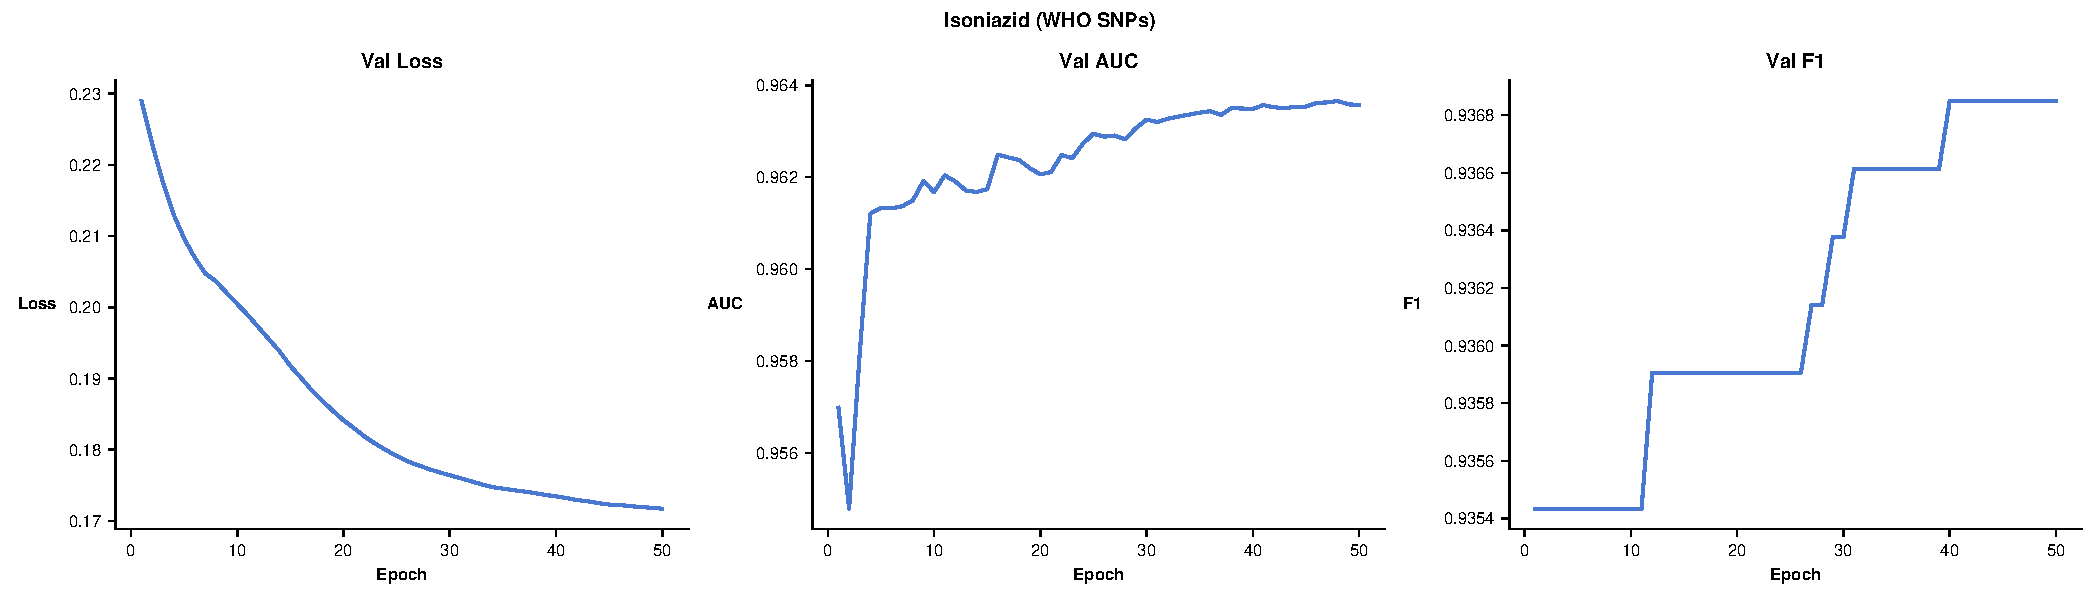
\includegraphics[width=\textwidth]{figures/who_isoniazid_learning_curves.pdf}
    \end{subfigure}
    \begin{subfigure}{\textwidth}
        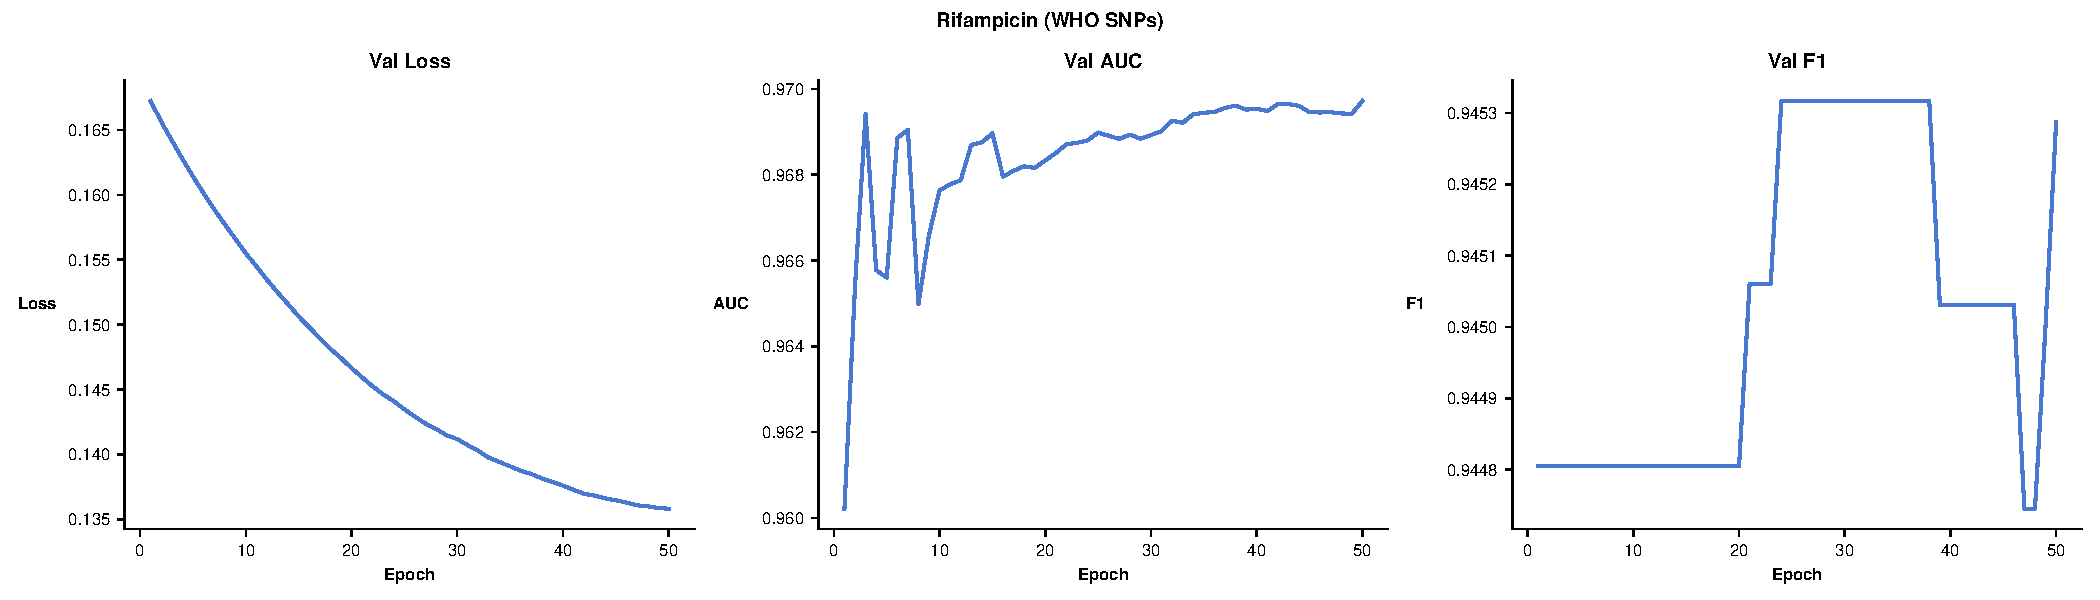
\includegraphics[width=\textwidth]{figures/who_rifampicin_learning_curves.pdf}
    \end{subfigure}
    \begin{subfigure}{\textwidth}
        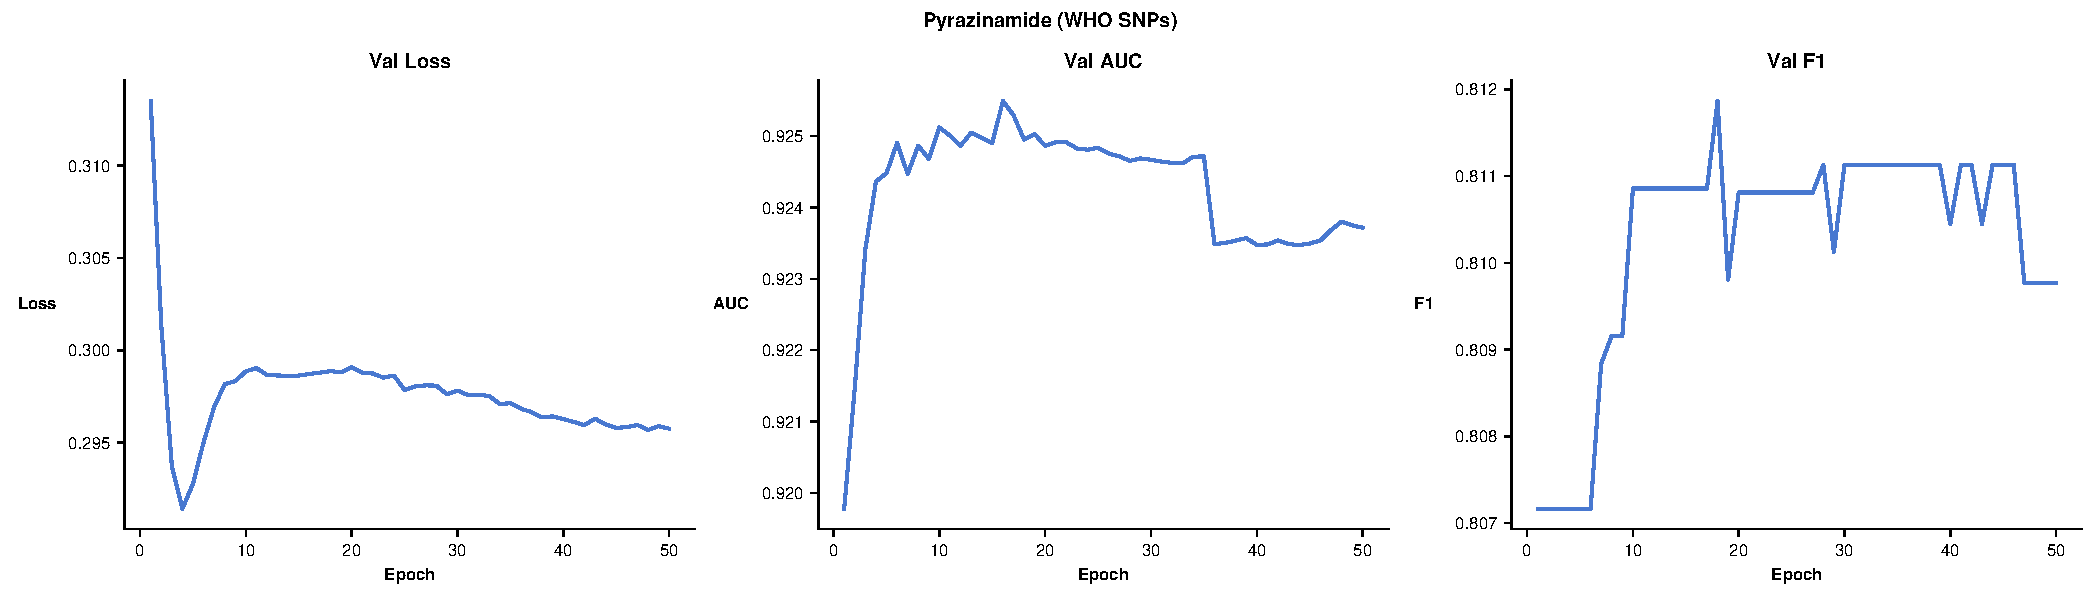
\includegraphics[width=\textwidth]{figures/who_pyrazinamide_learning_curves.pdf}
    \end{subfigure}
    \begin{subfigure}{\textwidth}
        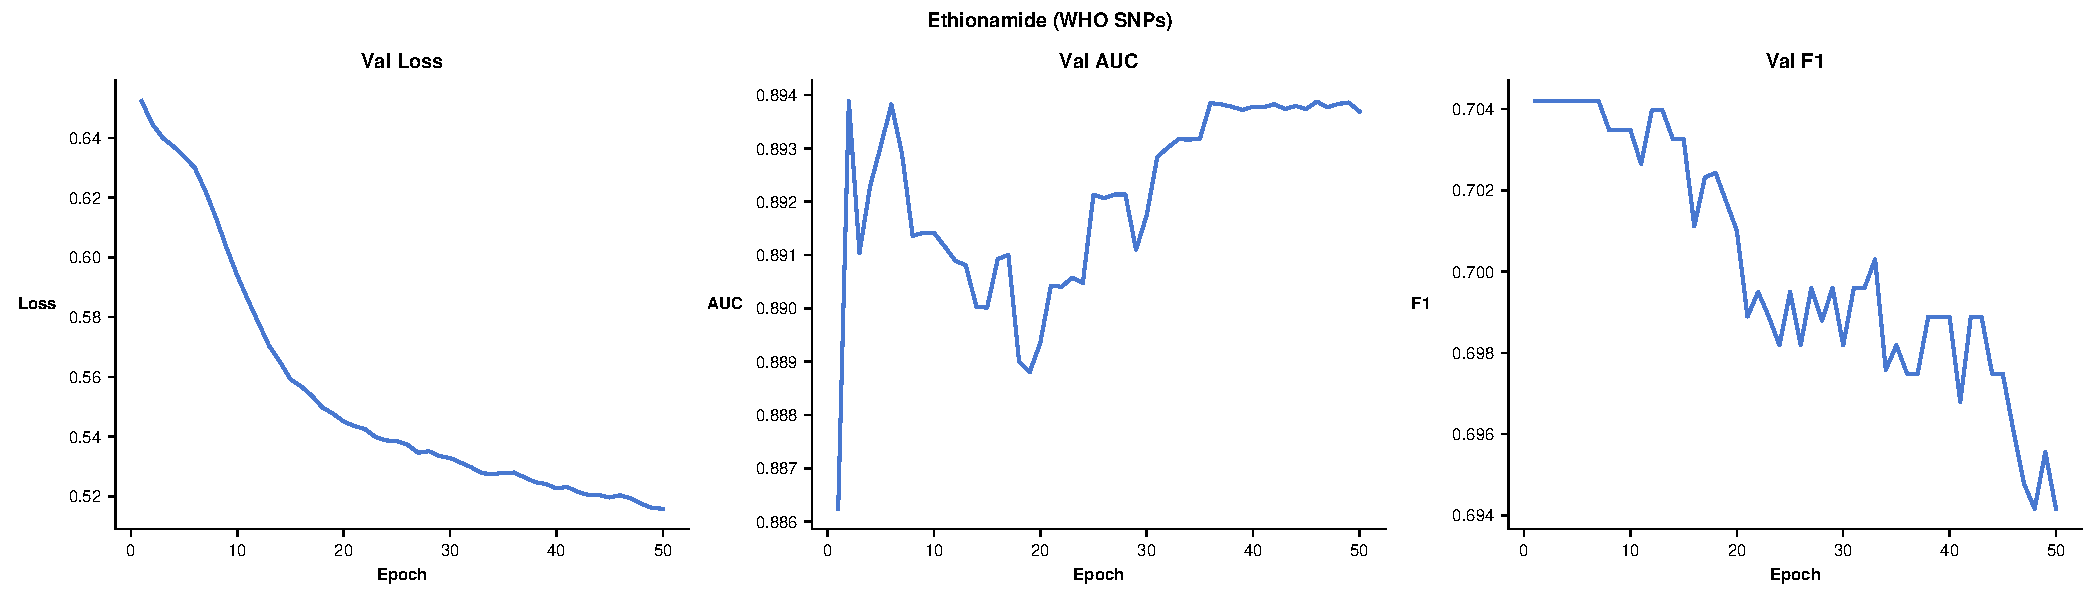
\includegraphics[width=\textwidth]{figures/who_ethionamide_learning_curves.pdf}
    \end{subfigure}
\end{figure}

\begin{figure}[H]
    \ContinuedFloat   % continues the same figure number
    \centering
    \begin{subfigure}{\textwidth}
        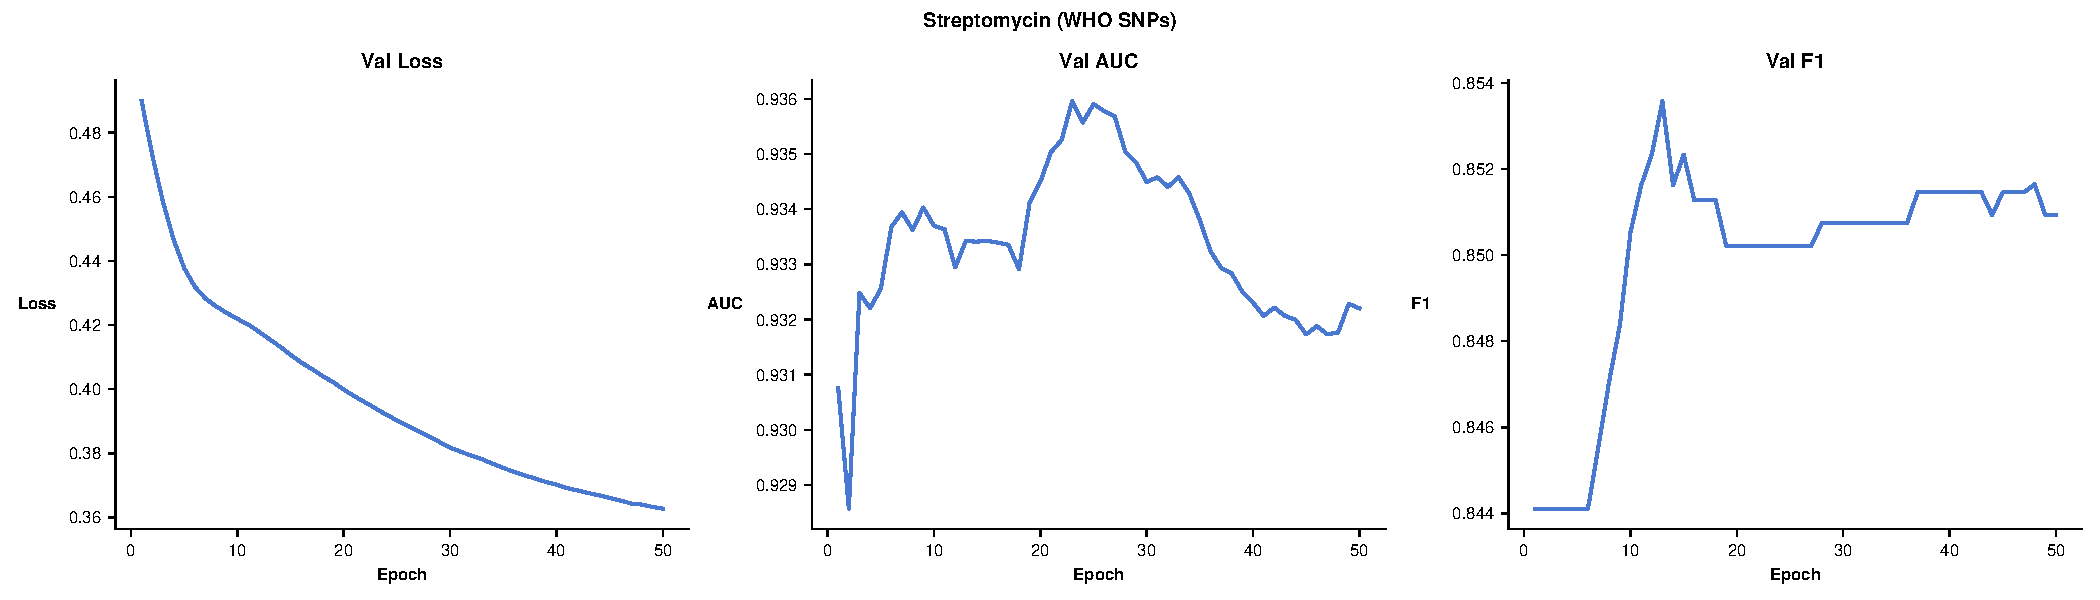
\includegraphics[width=\textwidth]{figures/who_streptomycin_learning_curves.pdf}
    \end{subfigure}
    \begin{subfigure}{\textwidth}
        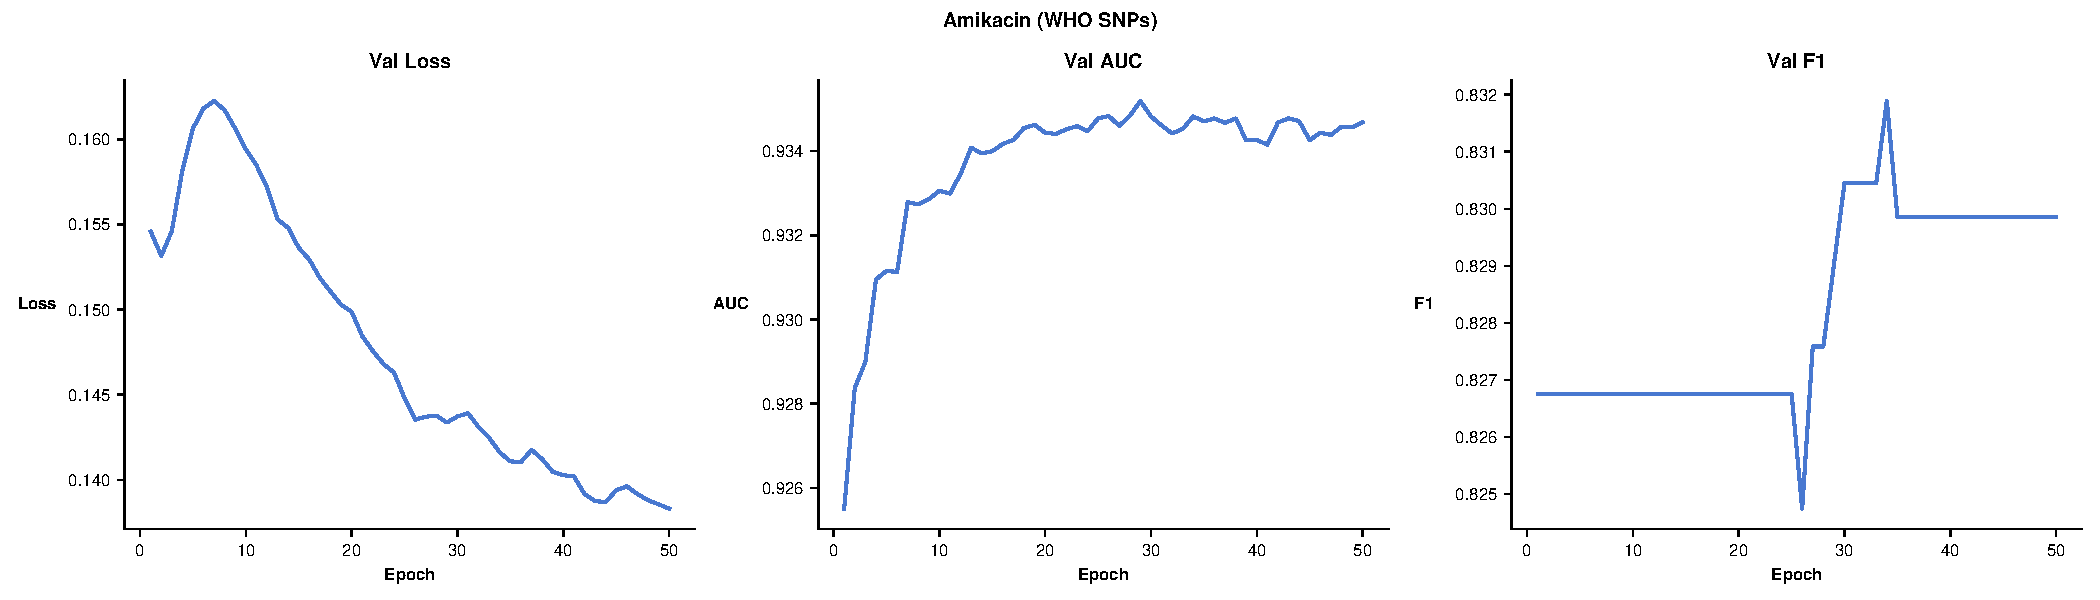
\includegraphics[width=\textwidth]{figures/who_amikacin_learning_curves.pdf}
    \end{subfigure}
    \begin{subfigure}{\textwidth}
        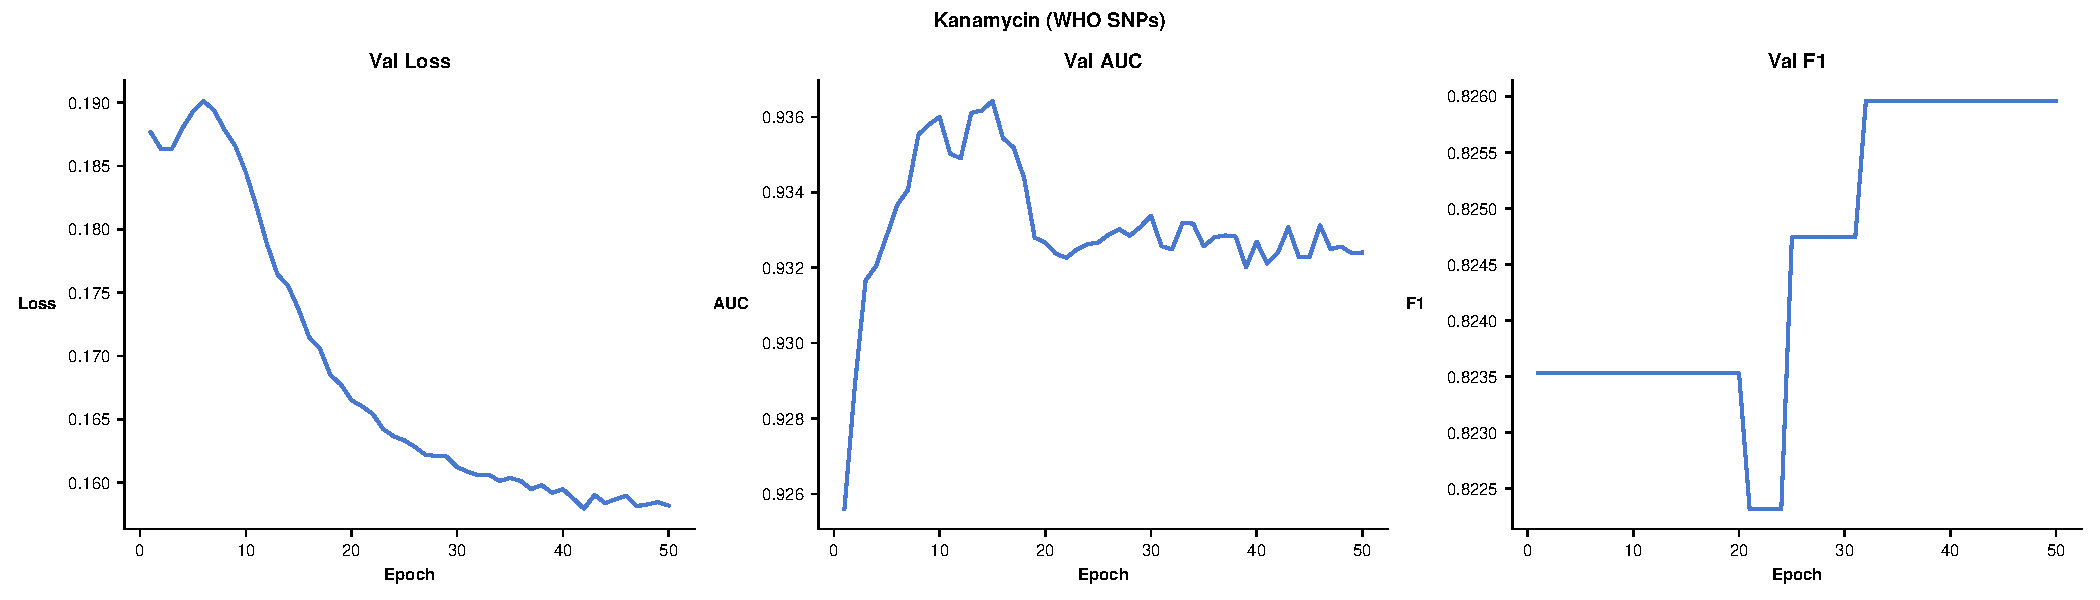
\includegraphics[width=\textwidth]{figures/who_kanamycin_learning_curves.pdf}
    \end{subfigure}
    \begin{subfigure}{\textwidth}
        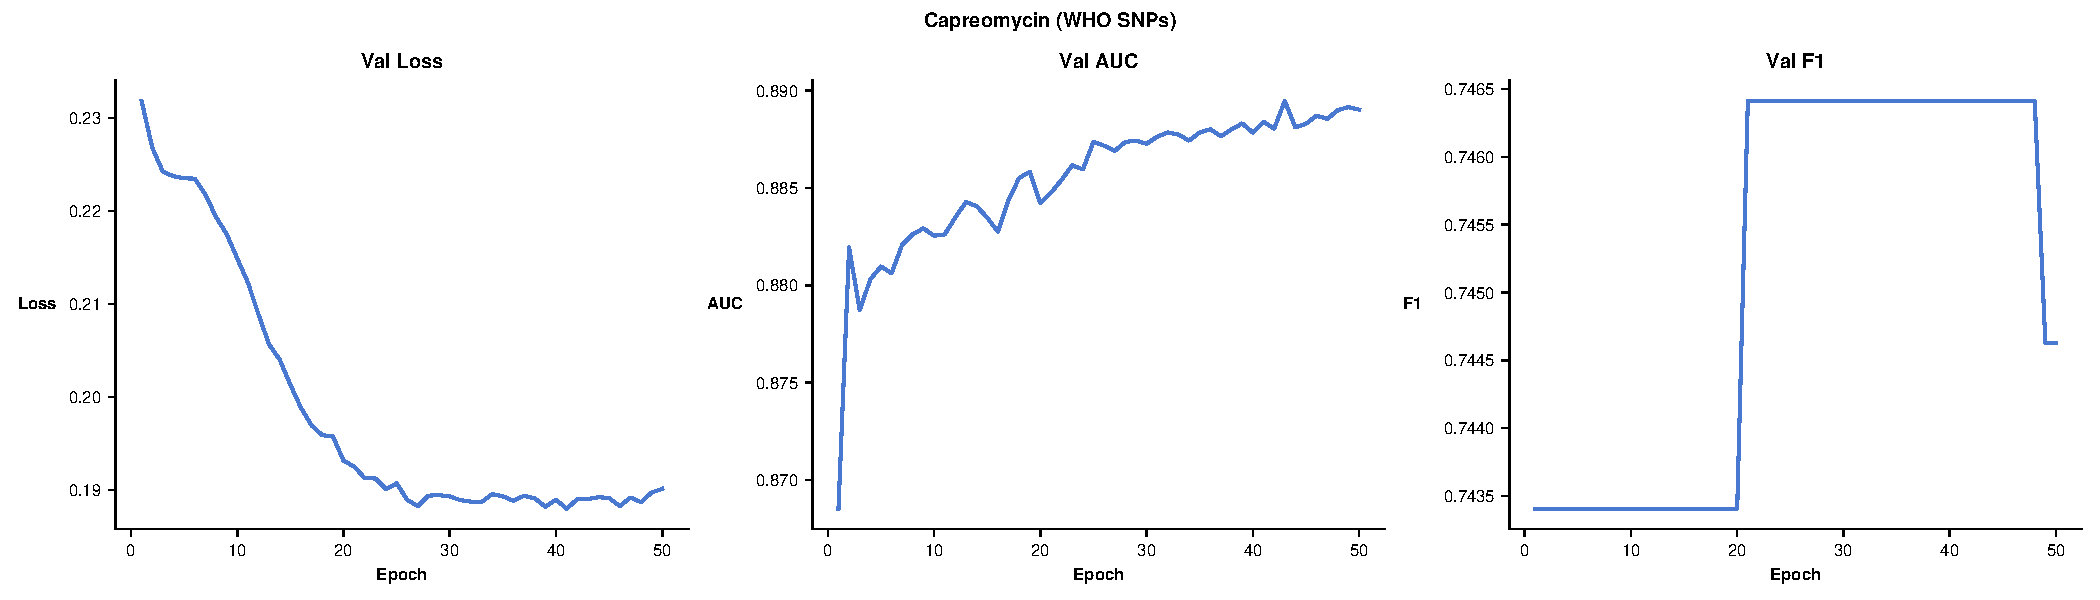
\includegraphics[width=\textwidth]{figures/who_capreomycin_learning_curves.pdf}
    \end{subfigure}
\end{figure}

\begin{figure}[H]
    \ContinuedFloat
    \centering
    \begin{subfigure}{\textwidth}
        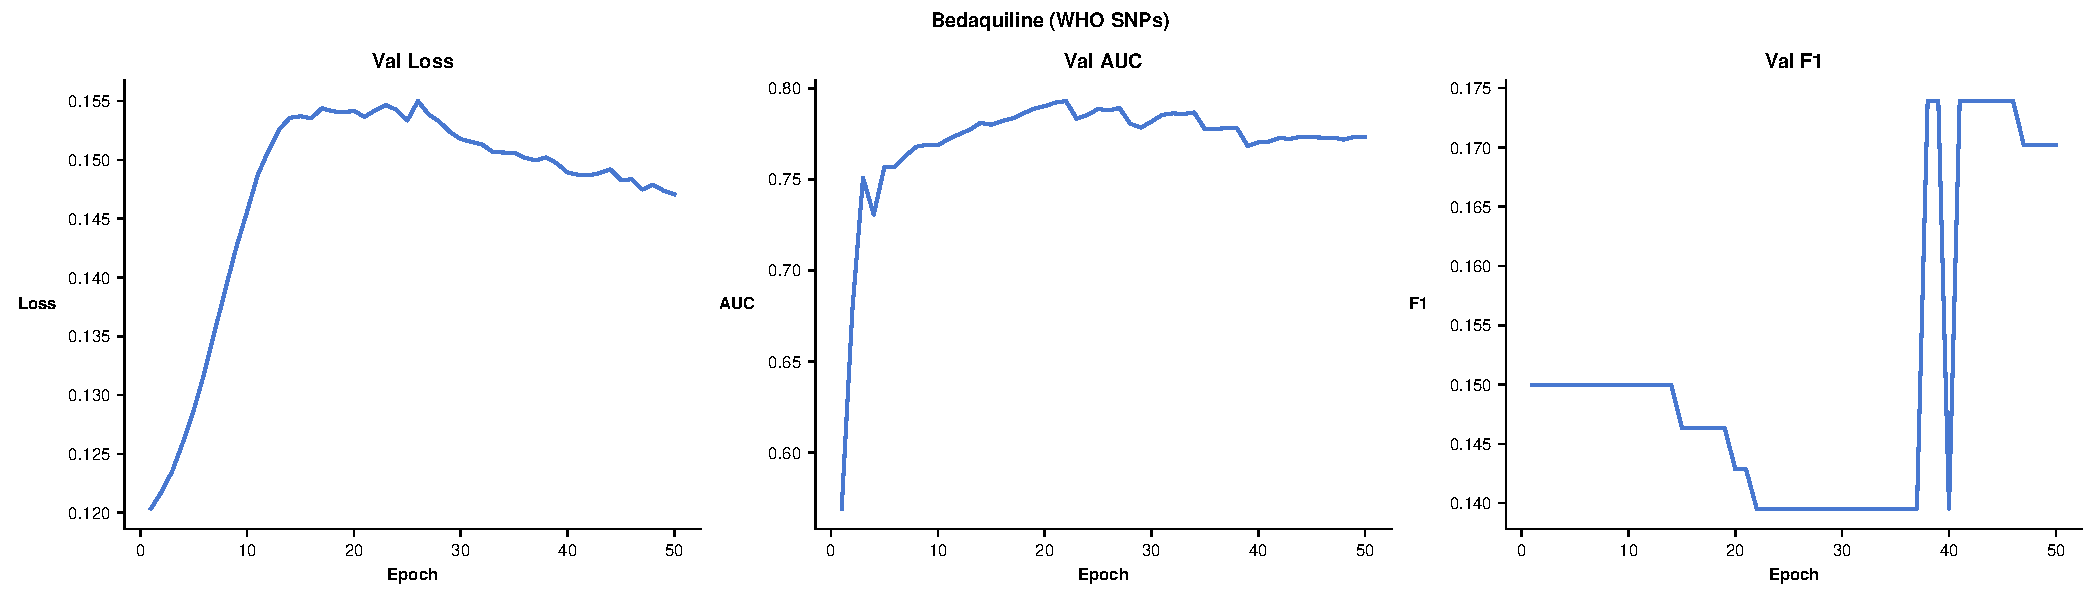
\includegraphics[width=\textwidth]{figures/who_bedaquiline_learning_curves.pdf}
    \end{subfigure}
    \begin{subfigure}{\textwidth}
        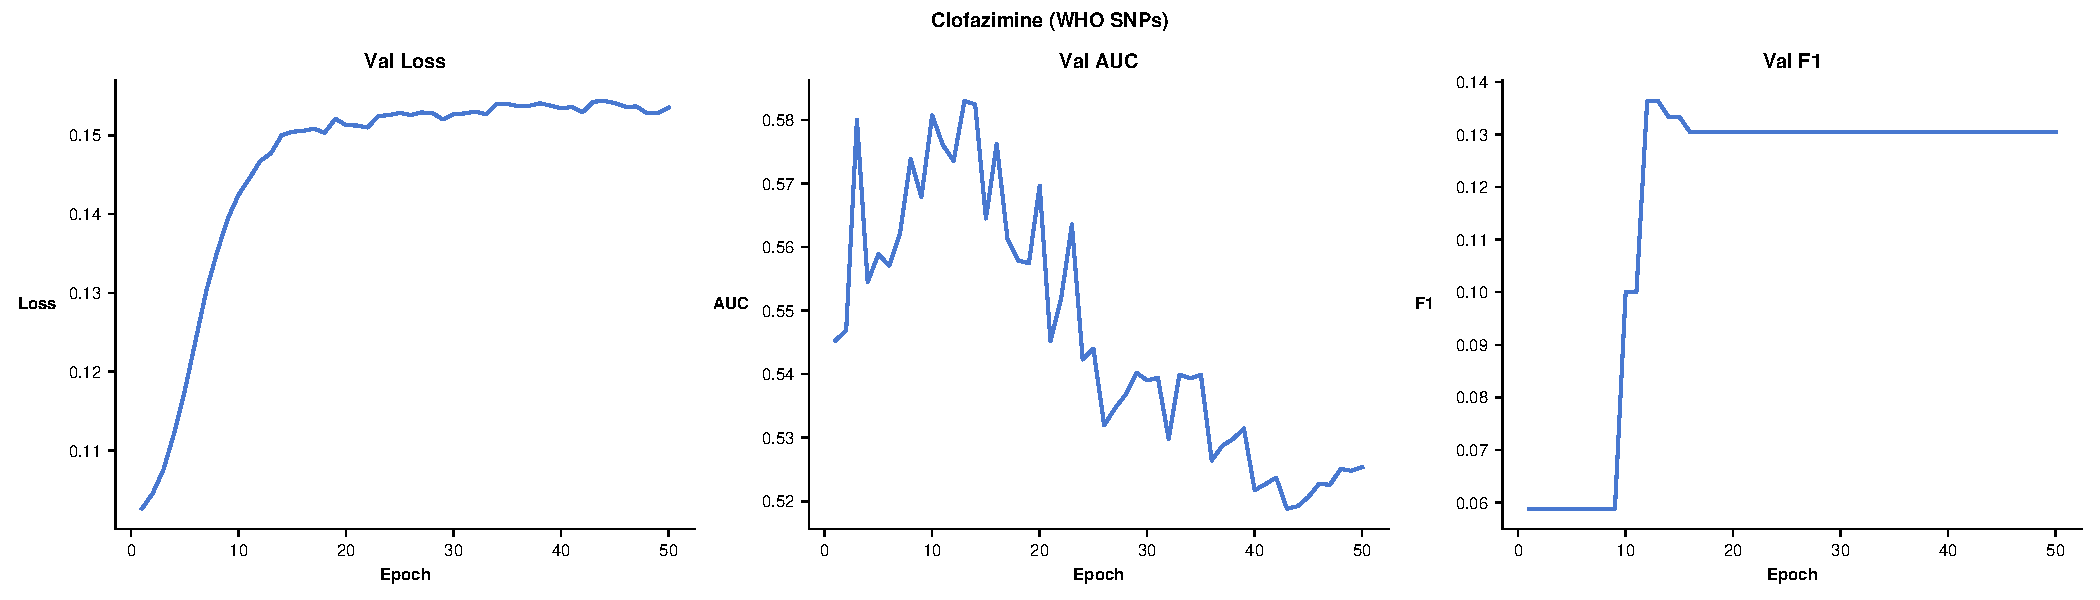
\includegraphics[width=\textwidth]{figures/who_clofazimine_learning_curves.pdf}
    \end{subfigure}
    \begin{subfigure}{\textwidth}
        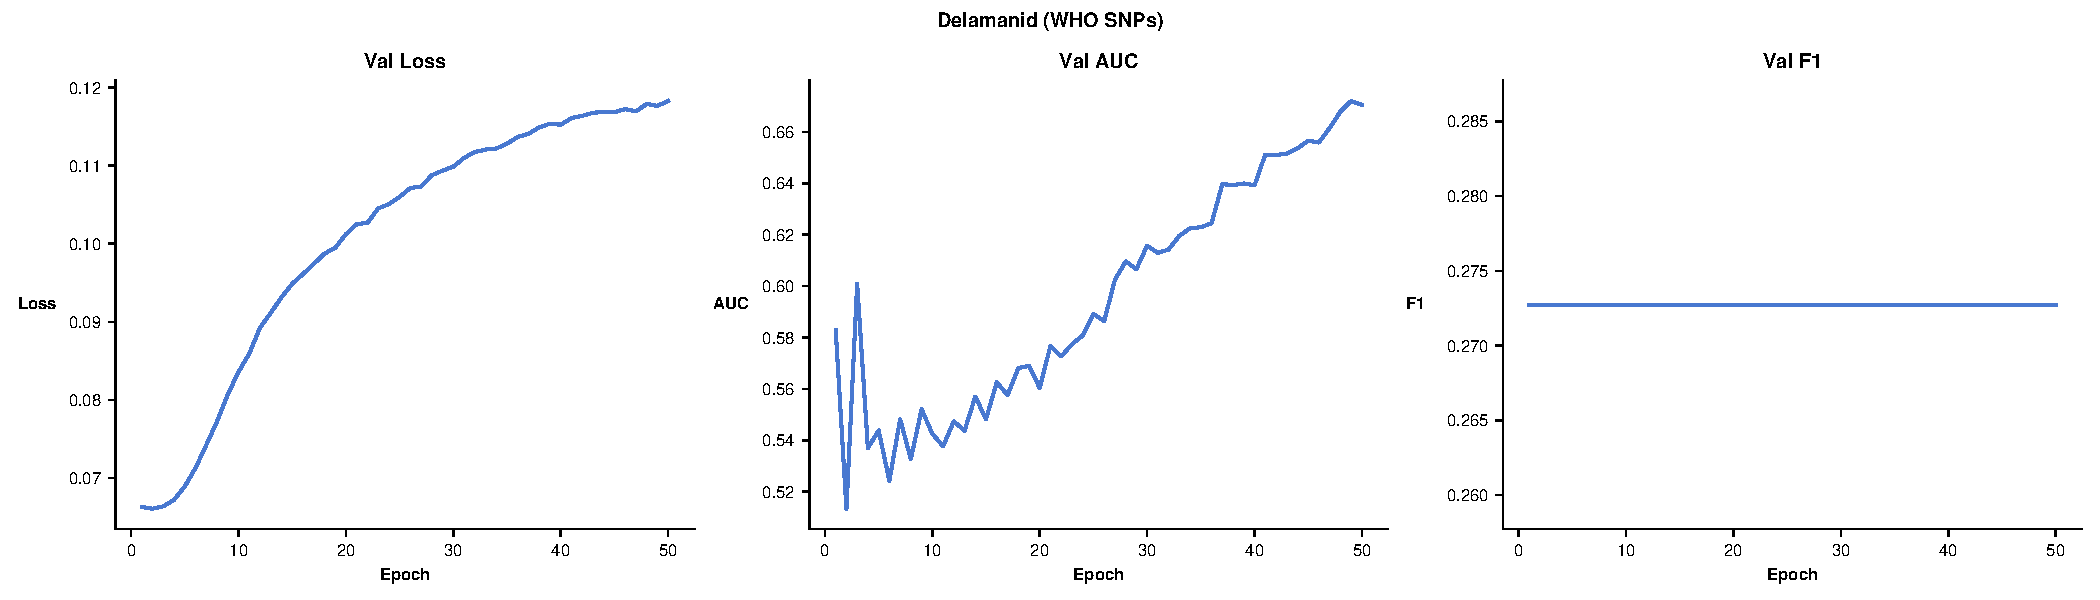
\includegraphics[width=\textwidth]{figures/who_delamanid_learning_curves.pdf}
    \end{subfigure}
    \begin{subfigure}{\textwidth}
        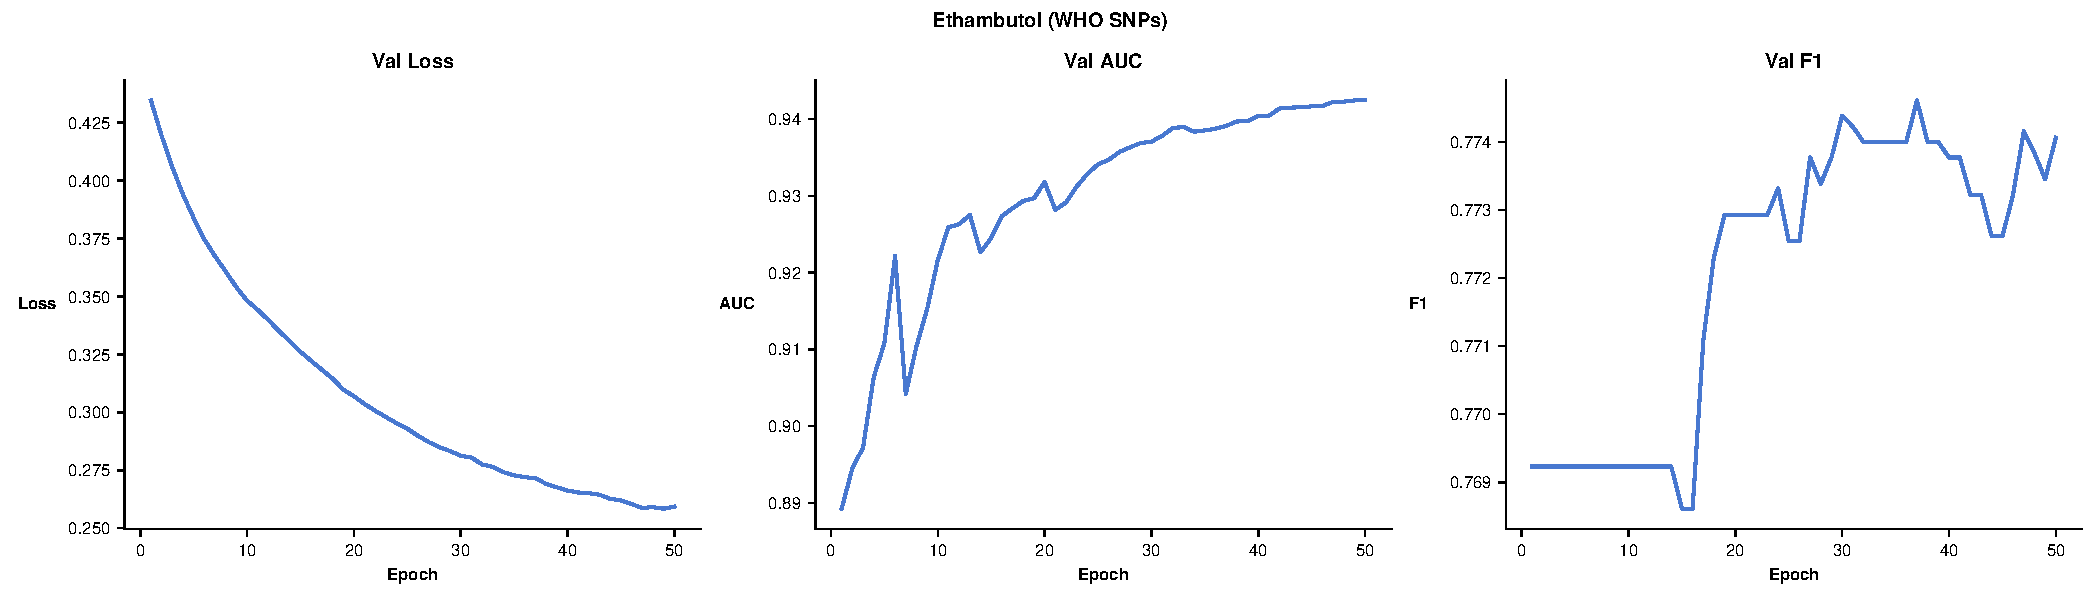
\includegraphics[width=\textwidth]{figures/who_ethambutol_learning_curves.pdf}
    \end{subfigure}
\end{figure}

\begin{figure}[H]
    \ContinuedFloat
    \centering
    \begin{subfigure}{\textwidth}
        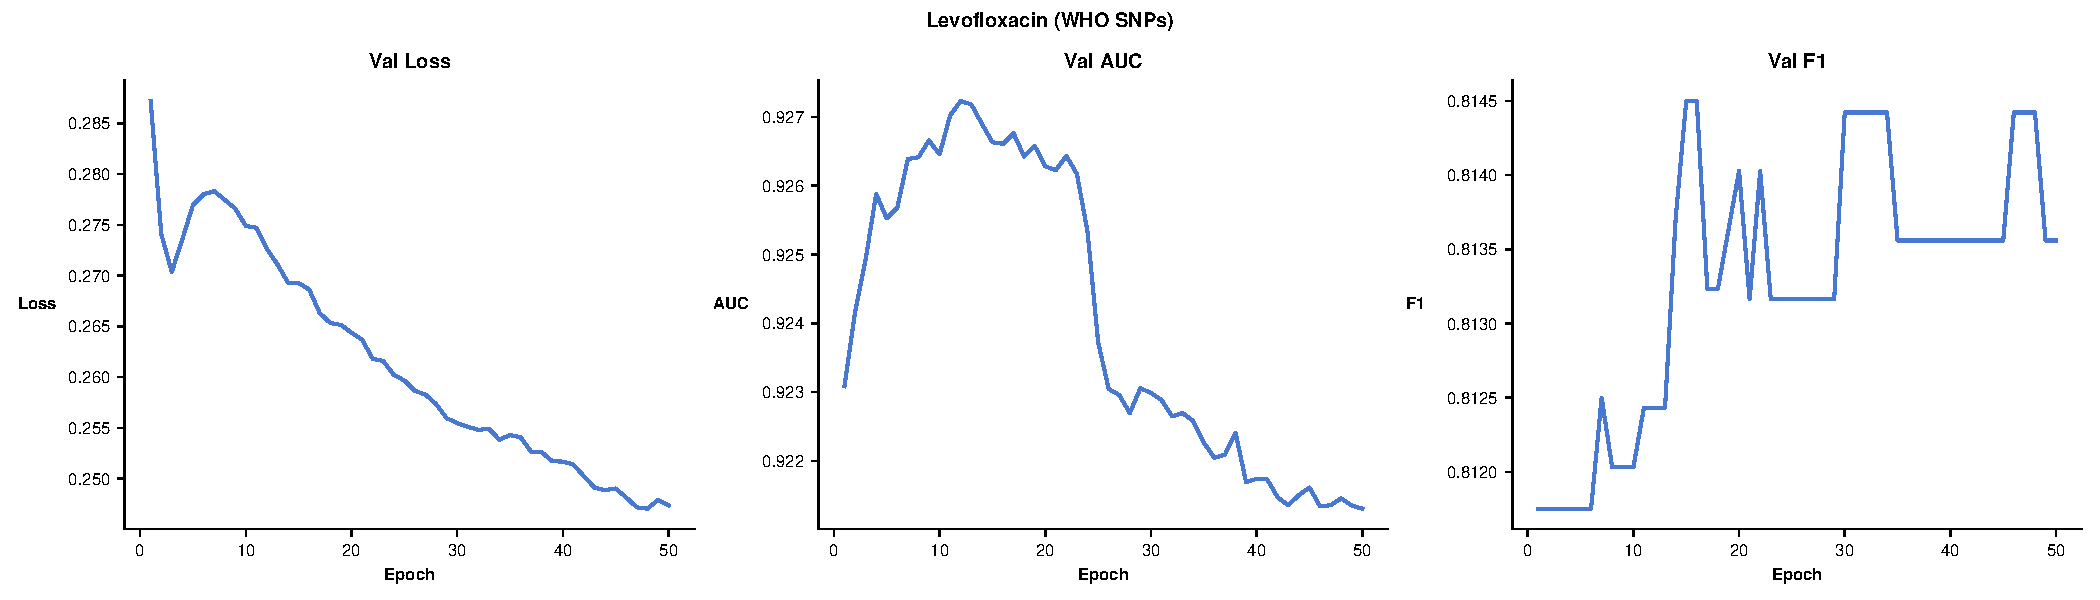
\includegraphics[width=\textwidth]{figures/who_levofloxacin_learning_curves.pdf}
    \end{subfigure}
    \begin{subfigure}{\textwidth}
        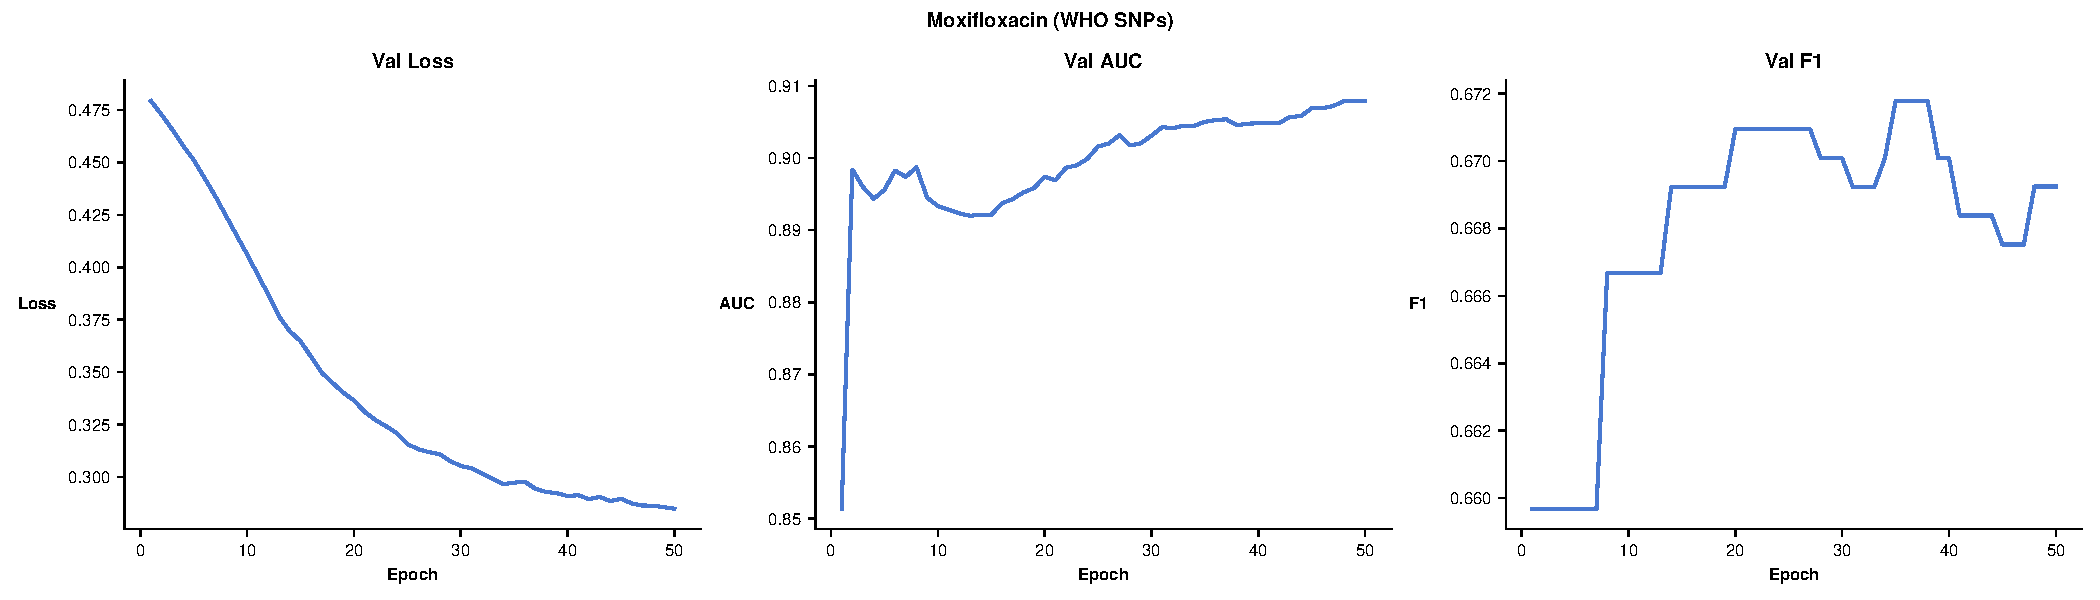
\includegraphics[width=\textwidth]{figures/who_moxifloxacin_learning_curves.pdf}
    \end{subfigure}
    \begin{subfigure}{\textwidth}
        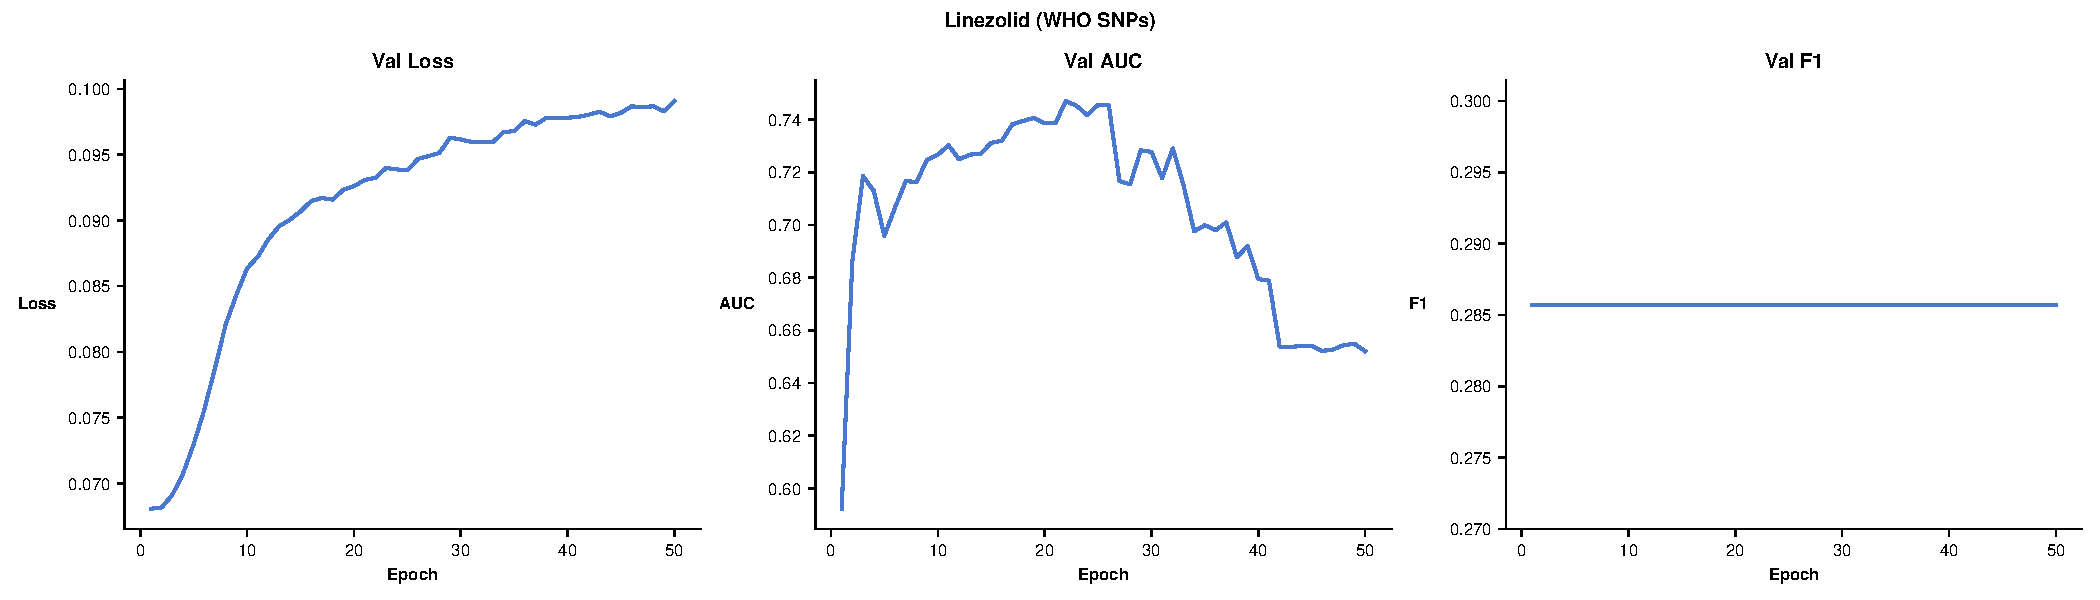
\includegraphics[width=\textwidth]{figures/who_linezolid_learning_curves.pdf}
    \end{subfigure}
    \caption{Model performance across all drugs}  % caption only on last block
    \label{fig:all_drugs}
\end{figure}

% Page 1
\begin{figure}[H]
    \centering
    \begin{subfigure}{\textwidth}
        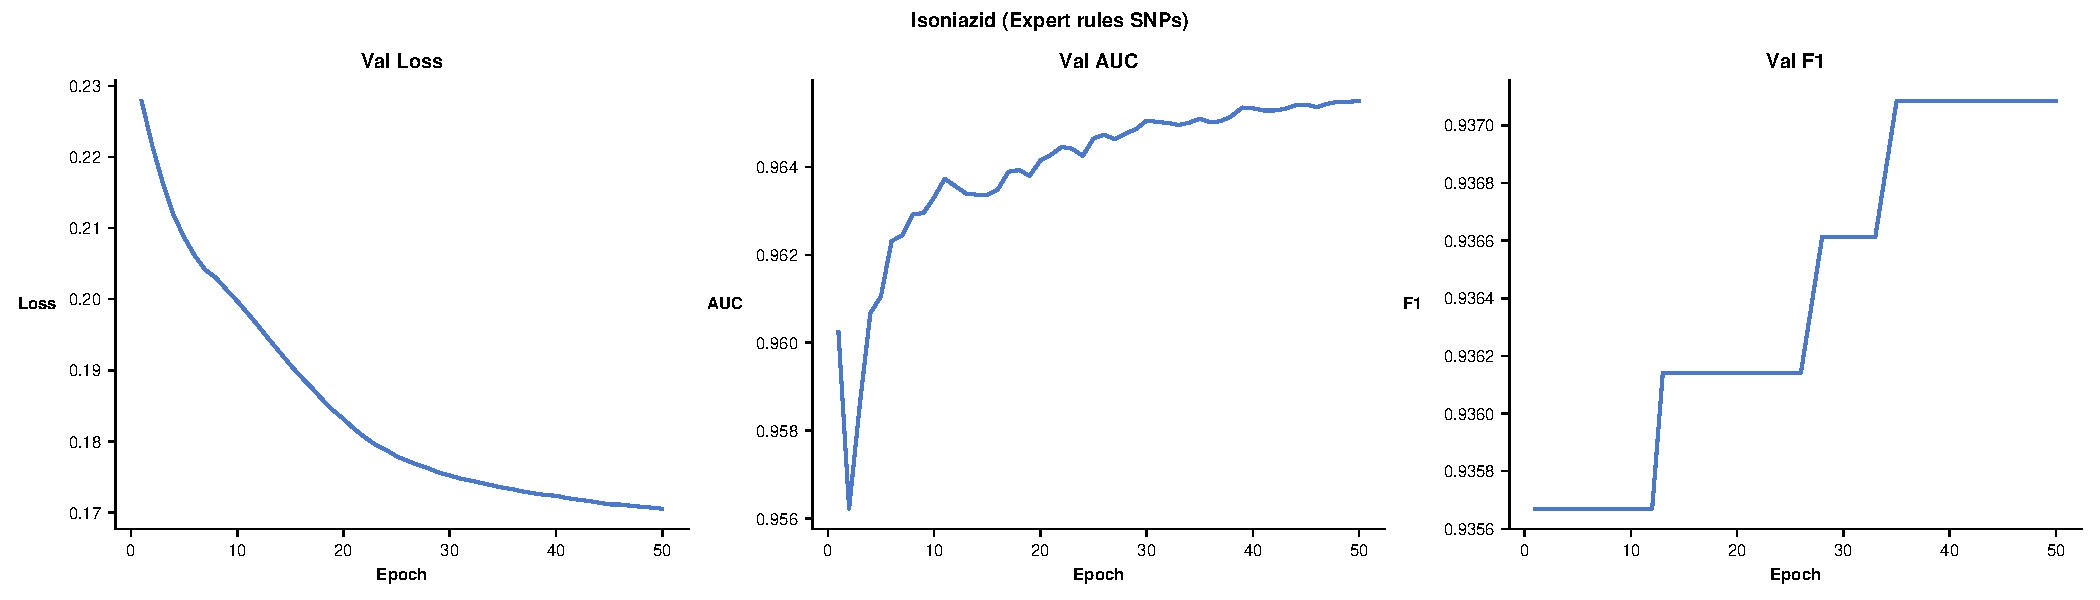
\includegraphics[width=\textwidth]{figures/expert_rules_isoniazid_learning_curves.pdf}
    \end{subfigure}
    \begin{subfigure}{\textwidth}
        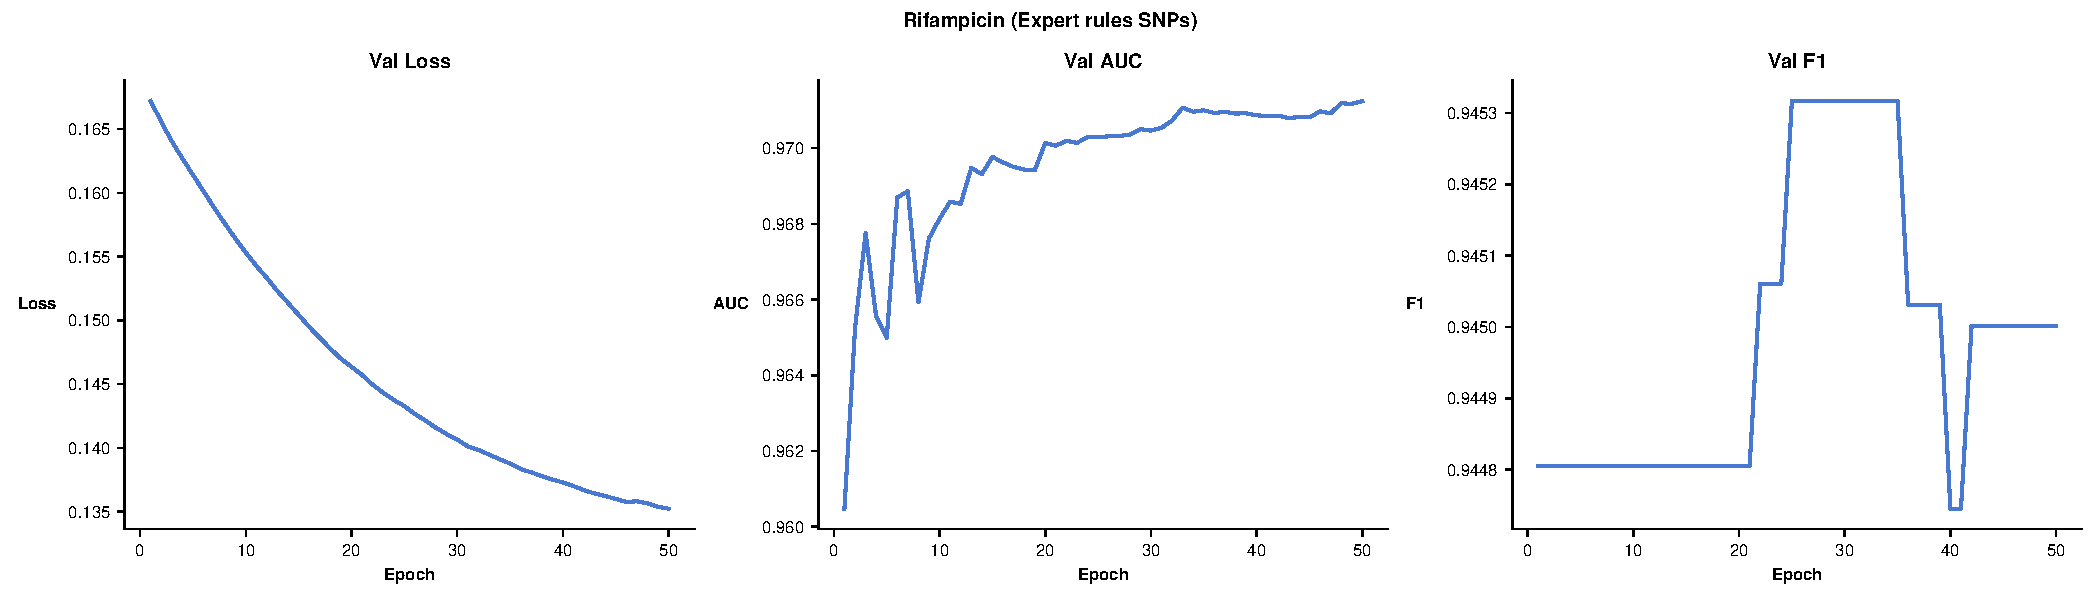
\includegraphics[width=\textwidth]{figures/expert_rules_rifampicin_learning_curves.pdf}
    \end{subfigure}
    \begin{subfigure}{\textwidth}
        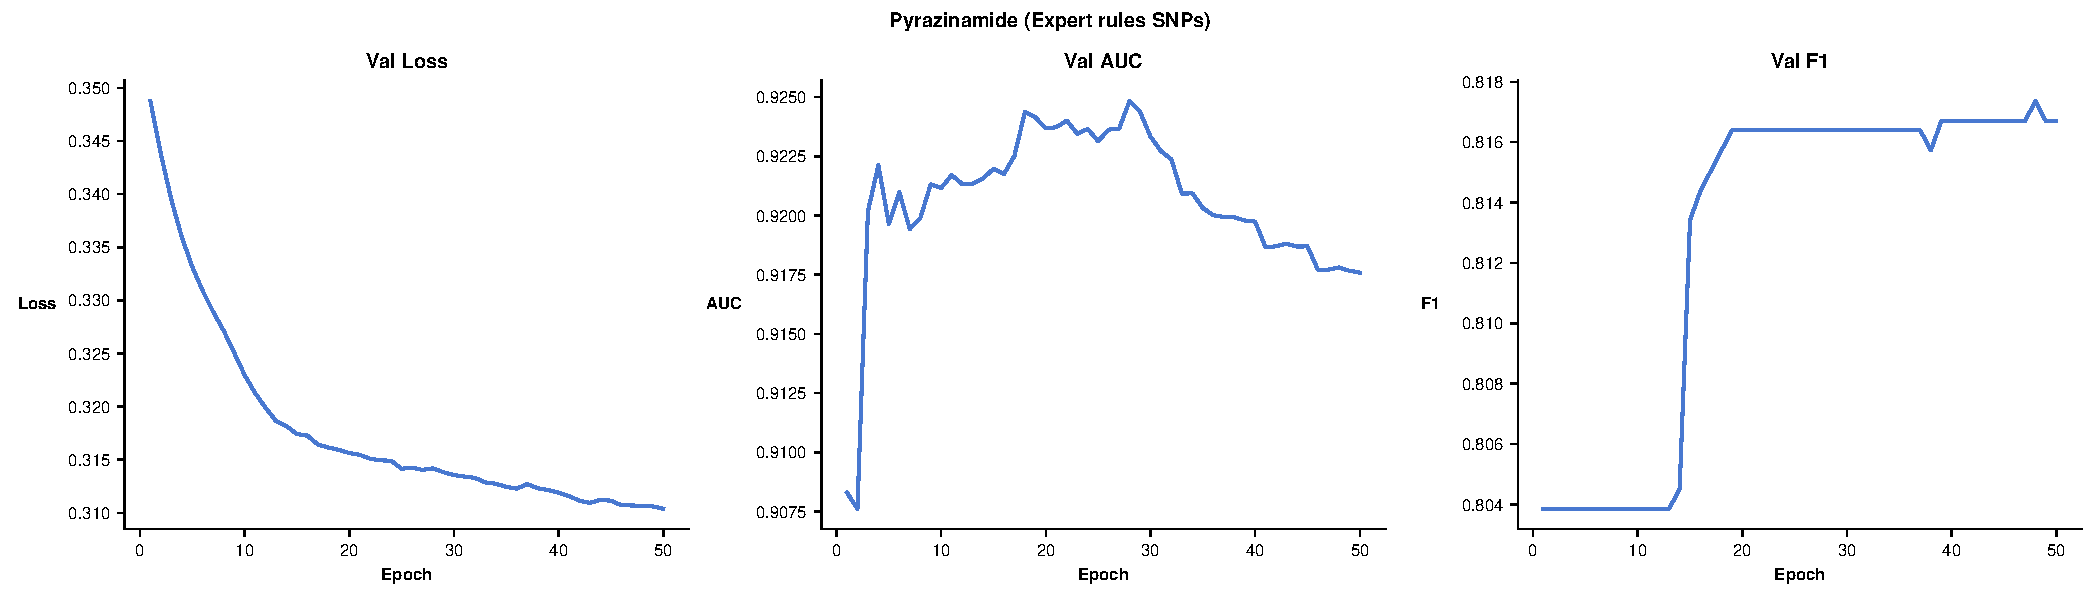
\includegraphics[width=\textwidth]{figures/expert_rules_pyrazinamide_learning_curves.pdf}
    \end{subfigure}
    \begin{subfigure}{\textwidth}
        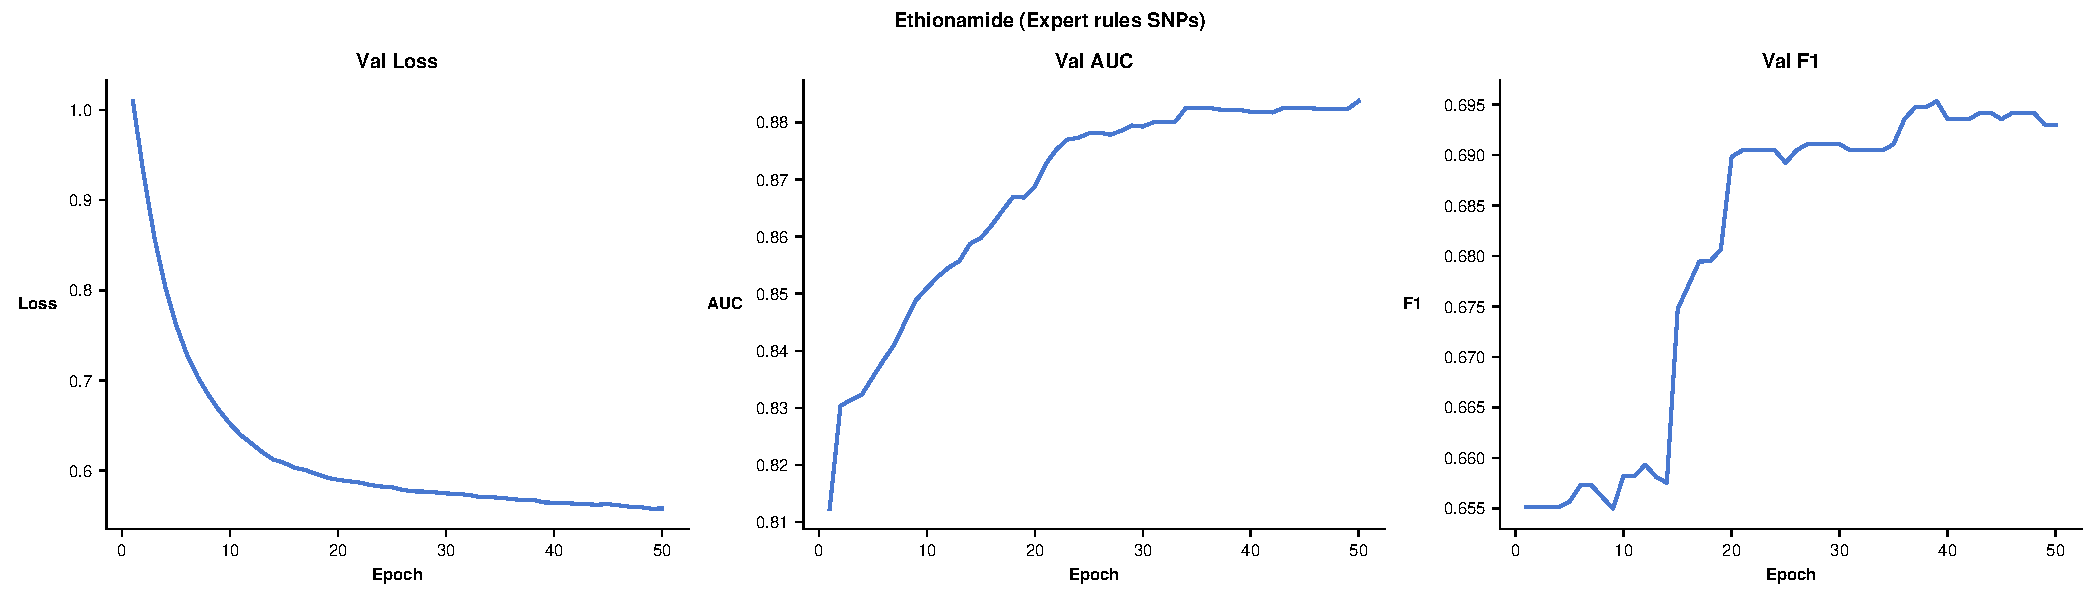
\includegraphics[width=\textwidth]{figures/expert_rules_ethionamide_learning_curves.pdf}
    \end{subfigure}
\end{figure}

\begin{figure}[H]
    \ContinuedFloat   % continues the same figure number
    \centering
    \begin{subfigure}{\textwidth}
        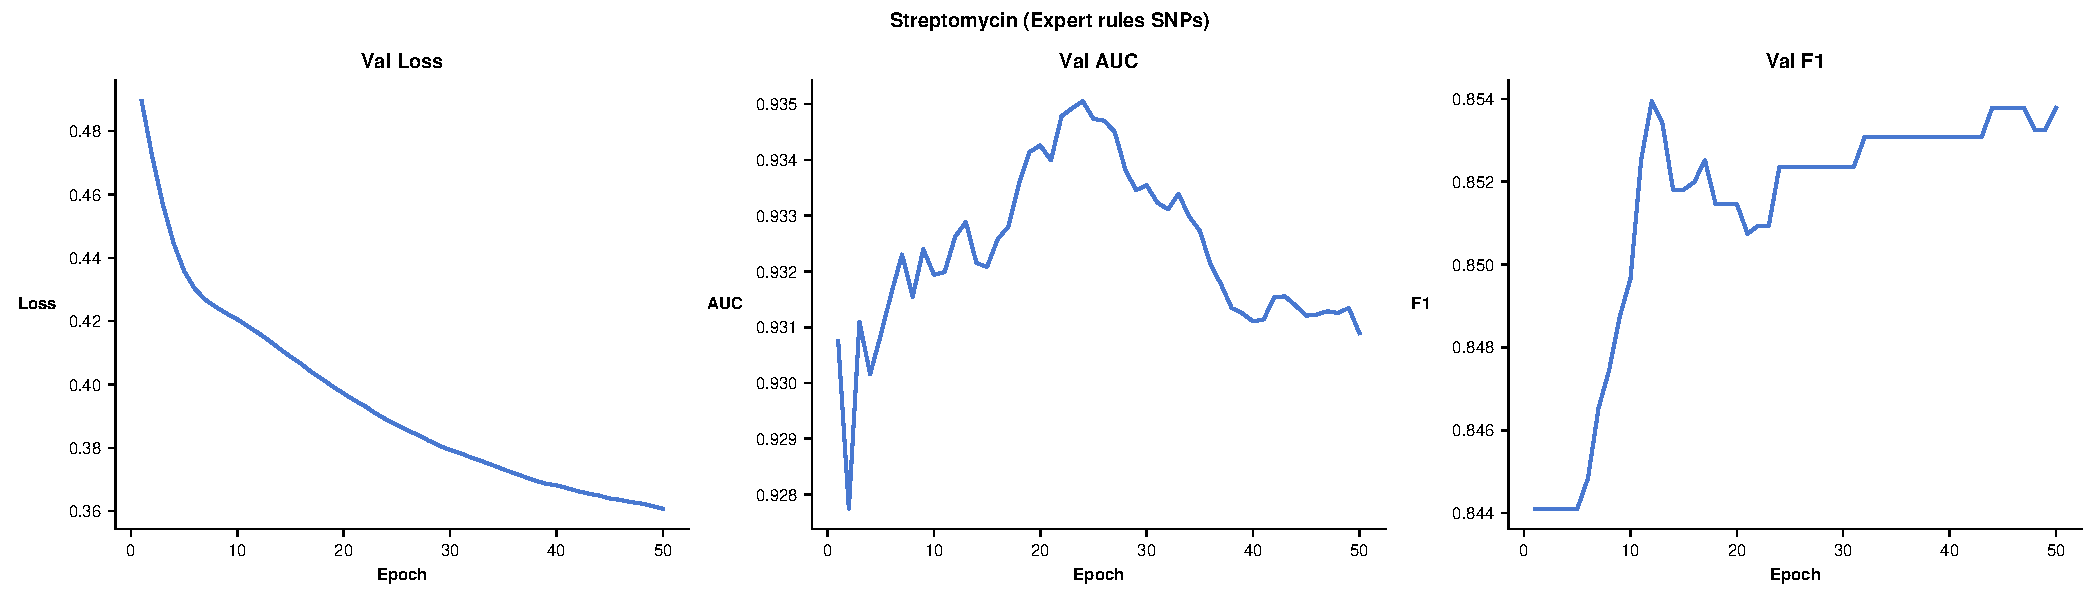
\includegraphics[width=\textwidth]{figures/expert_rules_streptomycin_learning_curves.pdf}
    \end{subfigure}
    \begin{subfigure}{\textwidth}
        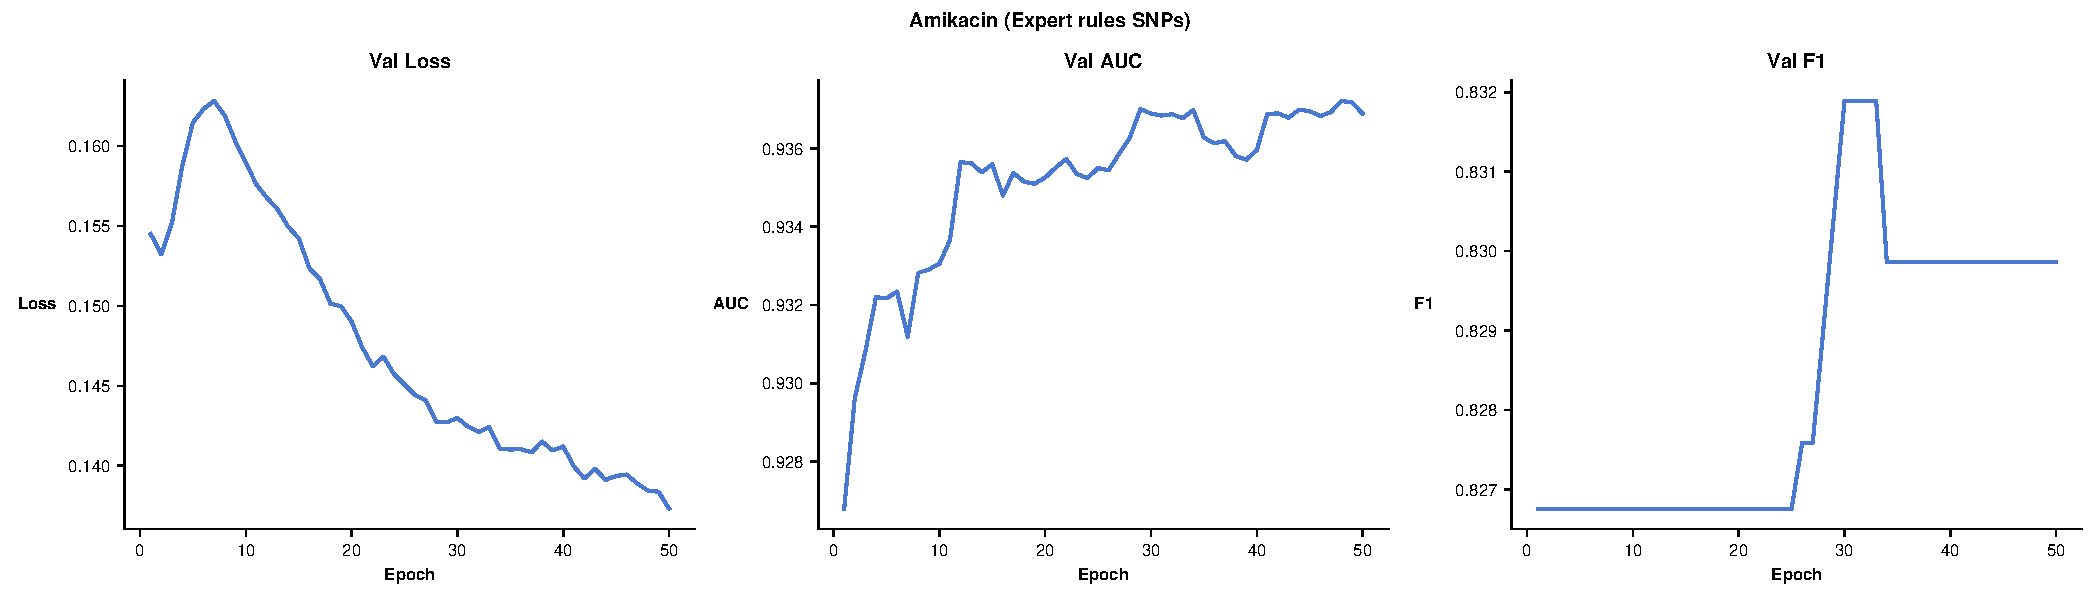
\includegraphics[width=\textwidth]{figures/expert_rules_amikacin_learning_curves.pdf}
    \end{subfigure}
    \begin{subfigure}{\textwidth}
        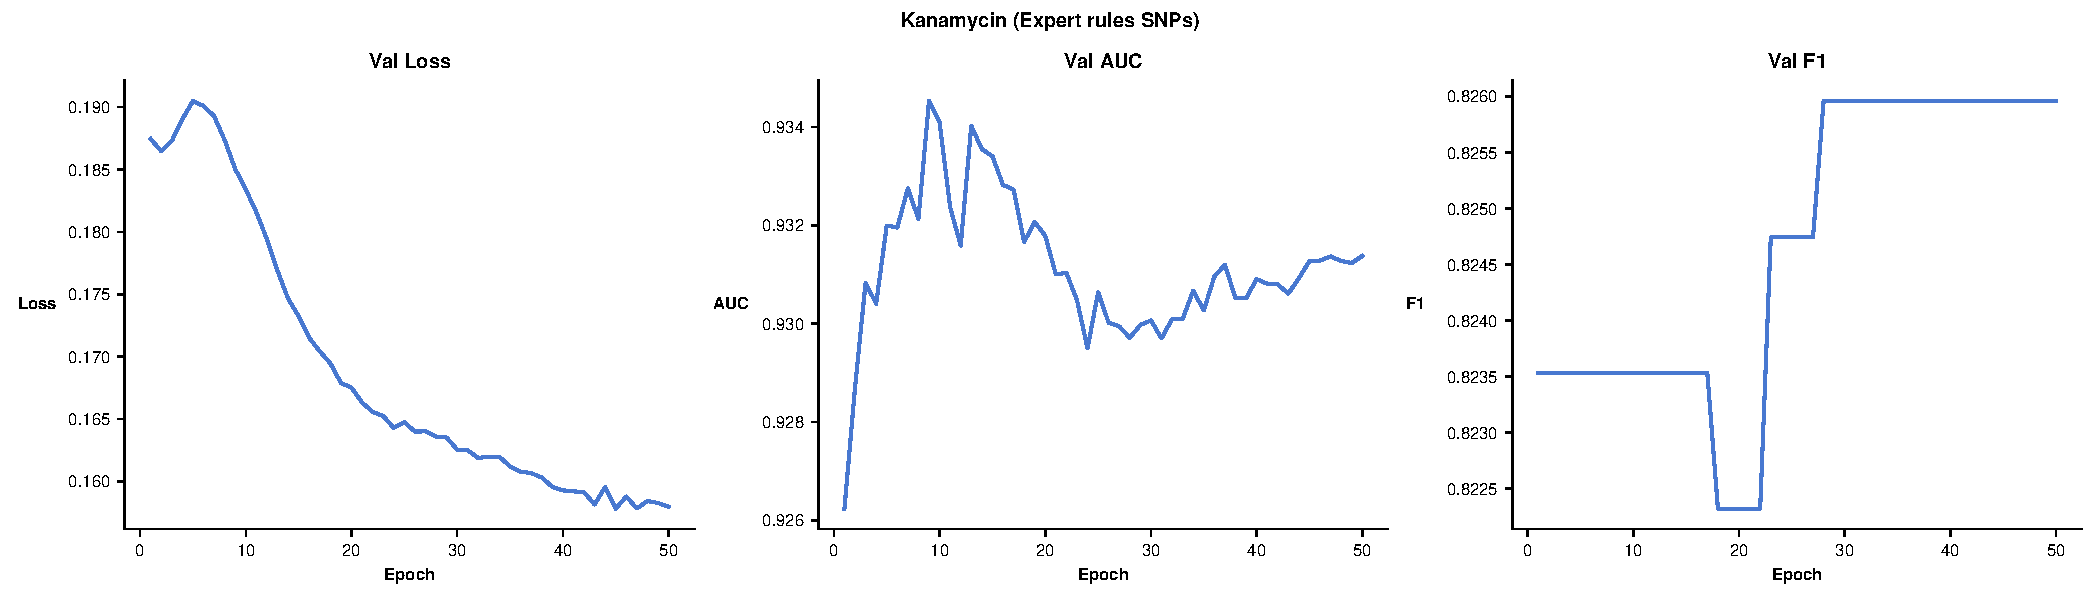
\includegraphics[width=\textwidth]{figures/expert_rules_kanamycin_learning_curves.pdf}
    \end{subfigure}
    \begin{subfigure}{\textwidth}
        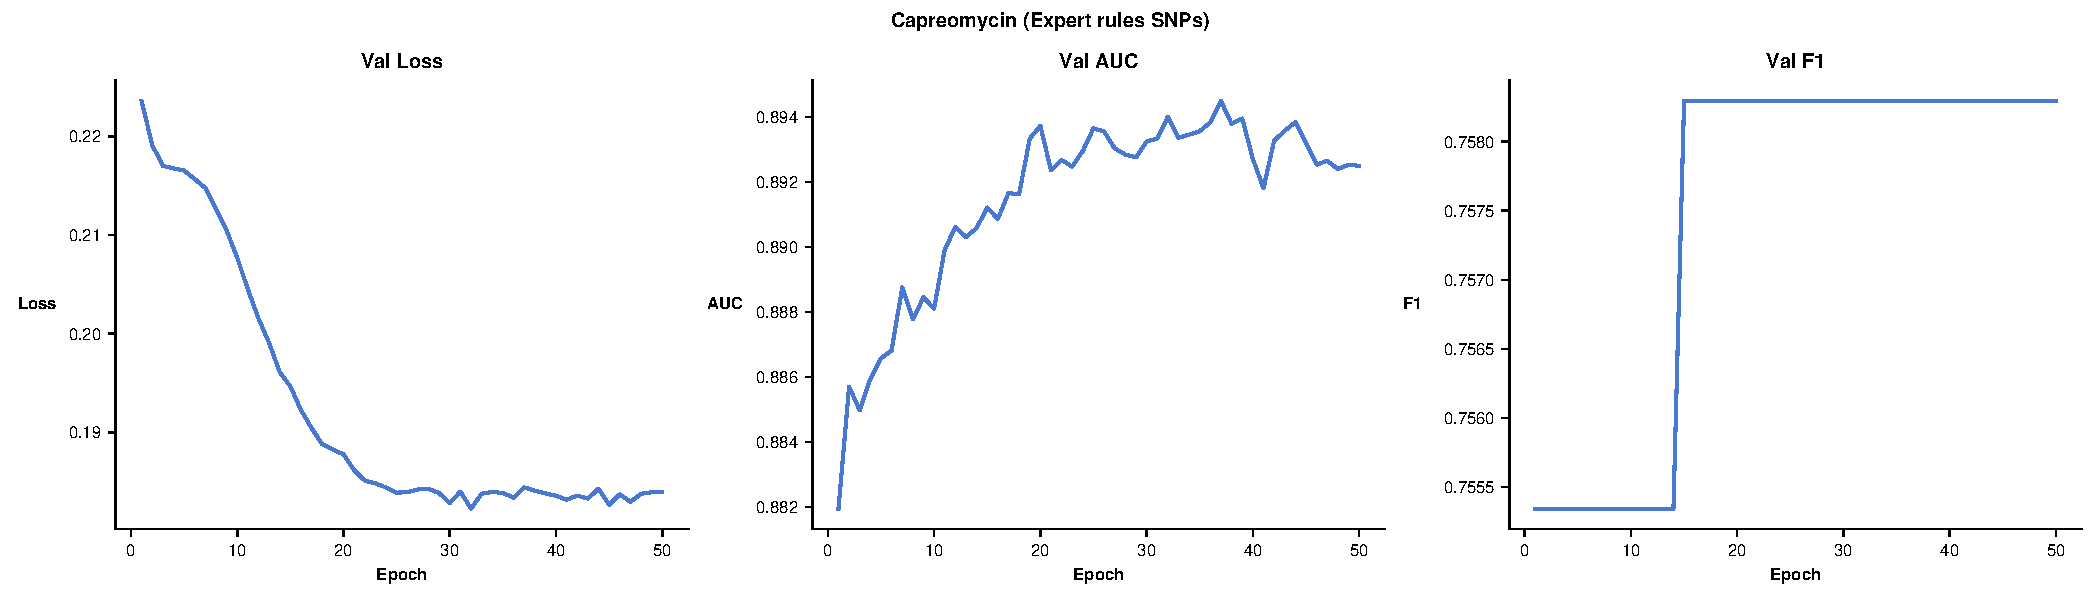
\includegraphics[width=\textwidth]{figures/expert_rules_capreomycin_learning_curves.pdf}
    \end{subfigure}
\end{figure}

\begin{figure}[H]
    \ContinuedFloat
    \centering
    \begin{subfigure}{\textwidth}
        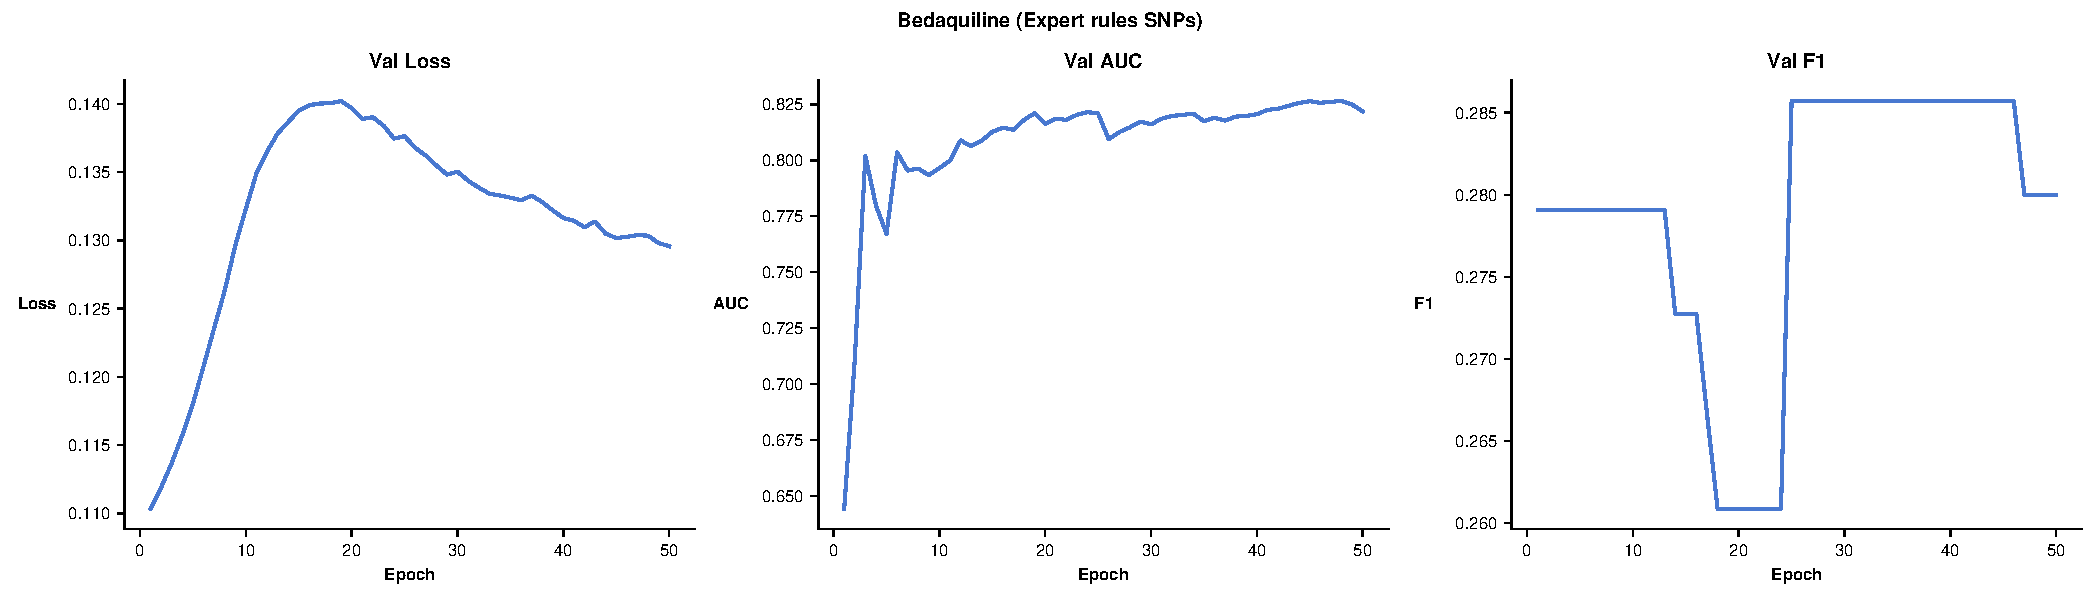
\includegraphics[width=\textwidth]{figures/expert_rules_bedaquiline_learning_curves.pdf}
    \end{subfigure}
    \begin{subfigure}{\textwidth}
        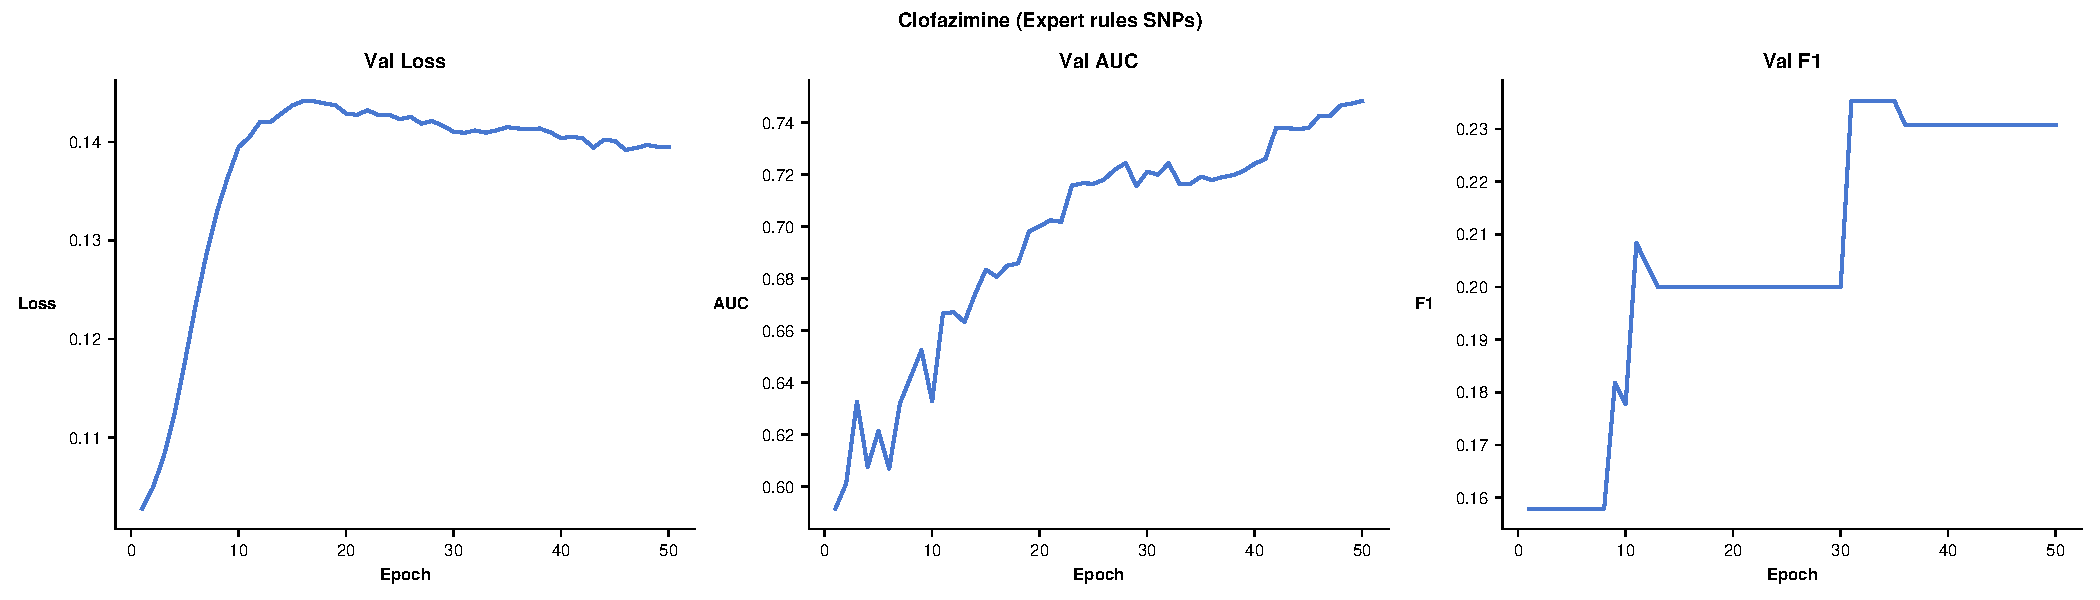
\includegraphics[width=\textwidth]{figures/expert_rules_clofazimine_learning_curves.pdf}
    \end{subfigure}
    \begin{subfigure}{\textwidth}
        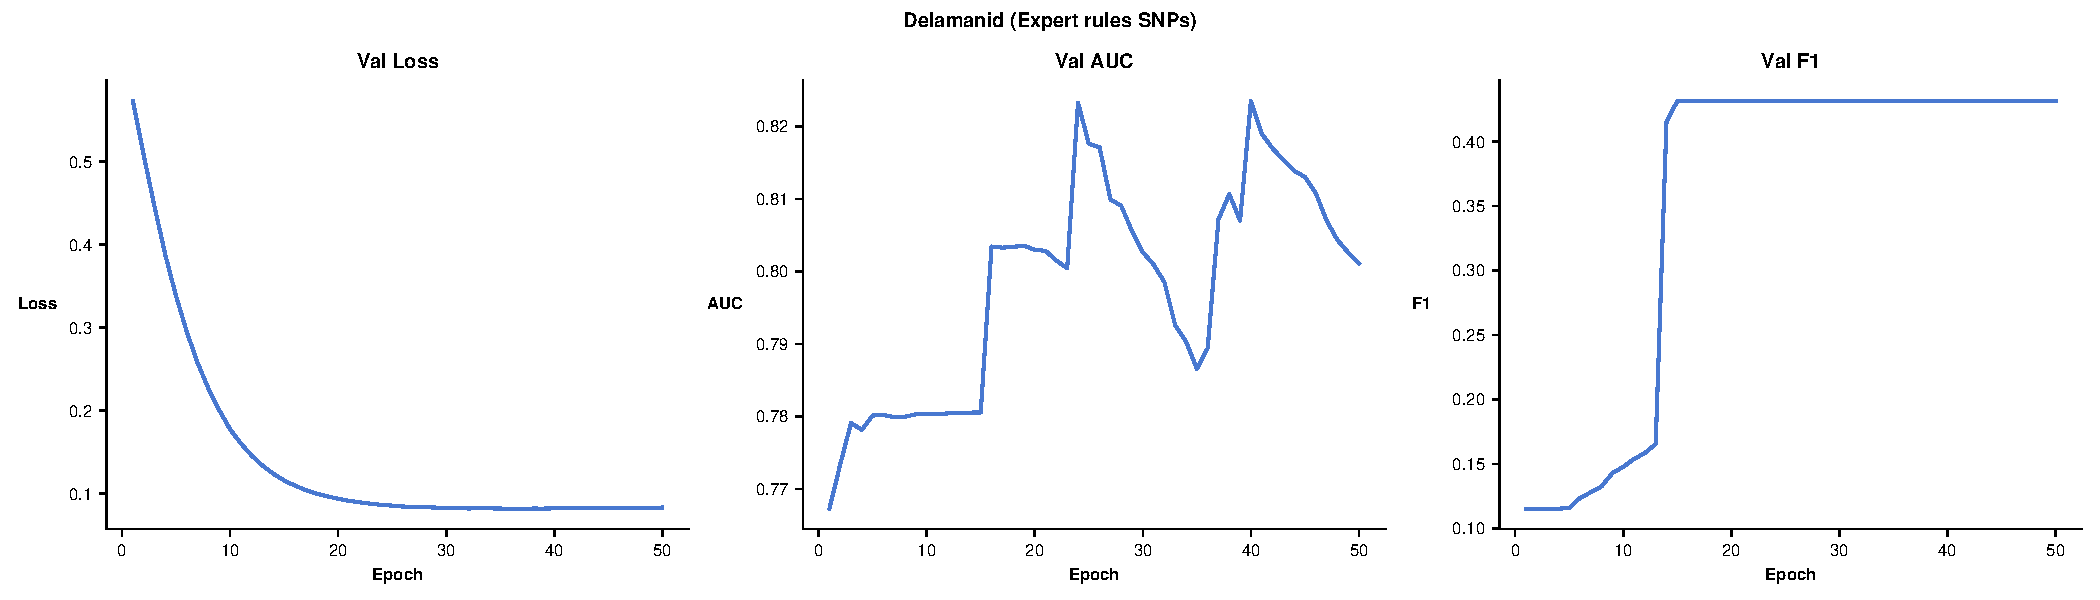
\includegraphics[width=\textwidth]{figures/expert_rules_delamanid_learning_curves.pdf}
    \end{subfigure}
    \begin{subfigure}{\textwidth}
        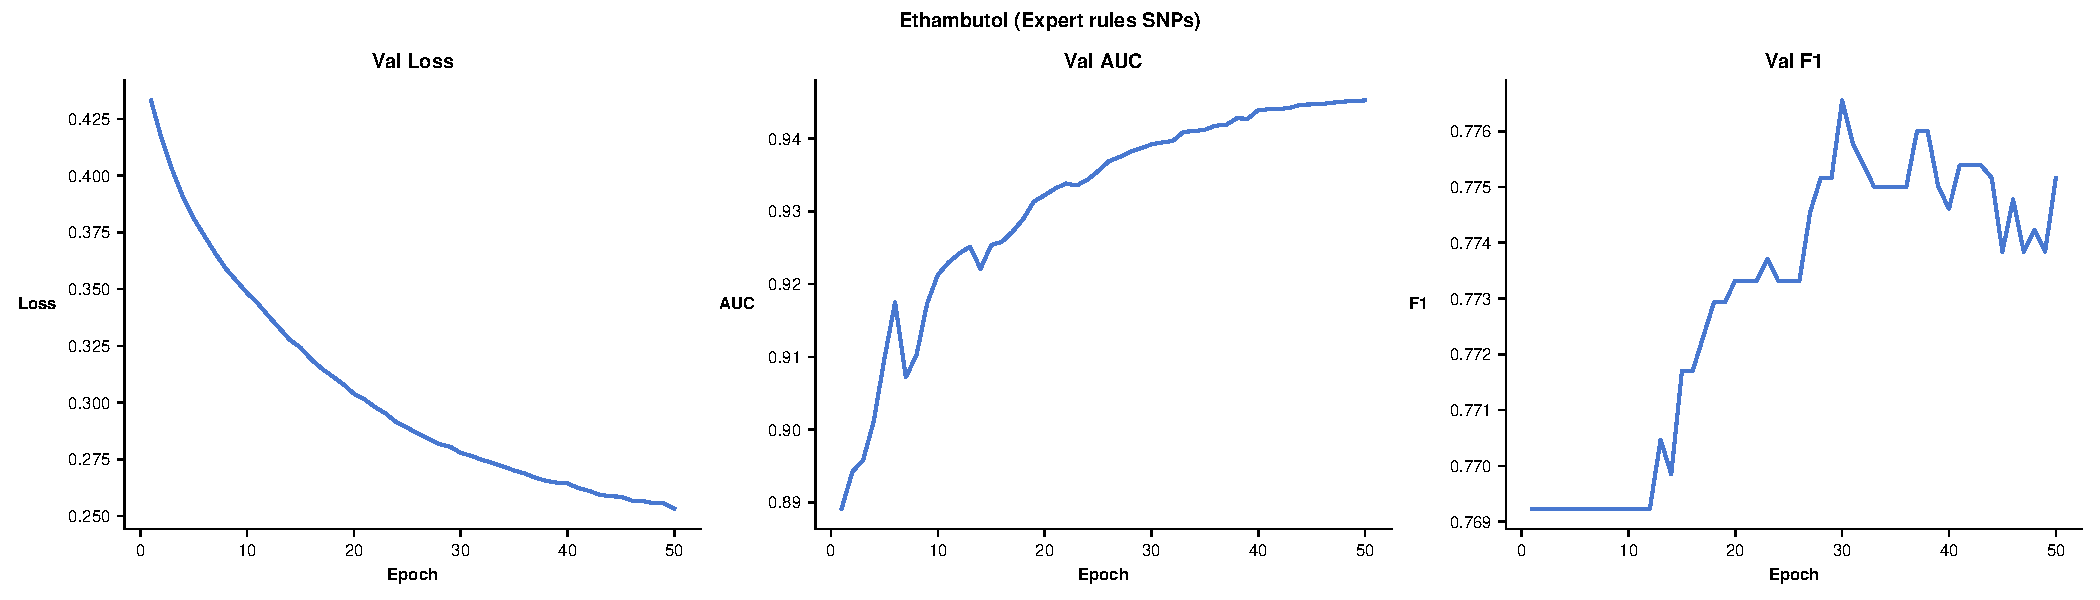
\includegraphics[width=\textwidth]{figures/expert_rules_ethambutol_learning_curves.pdf}
    \end{subfigure}
\end{figure}

\begin{figure}[H]
    \ContinuedFloat
    \centering
    \begin{subfigure}{\textwidth}
        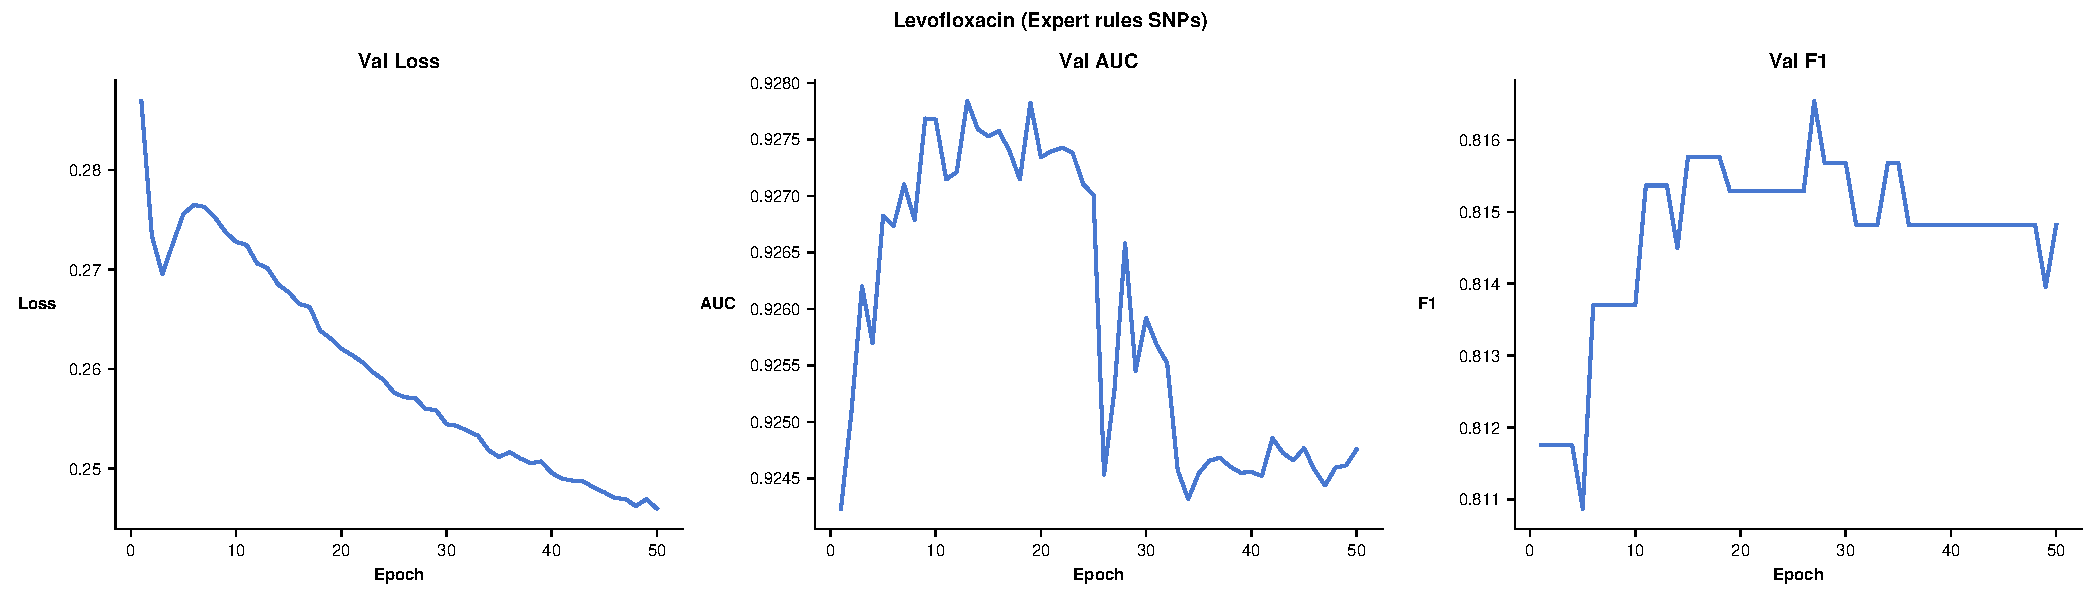
\includegraphics[width=\textwidth]{figures/expert_rules_levofloxacin_learning_curves.pdf}
    \end{subfigure}
    \begin{subfigure}{\textwidth}
        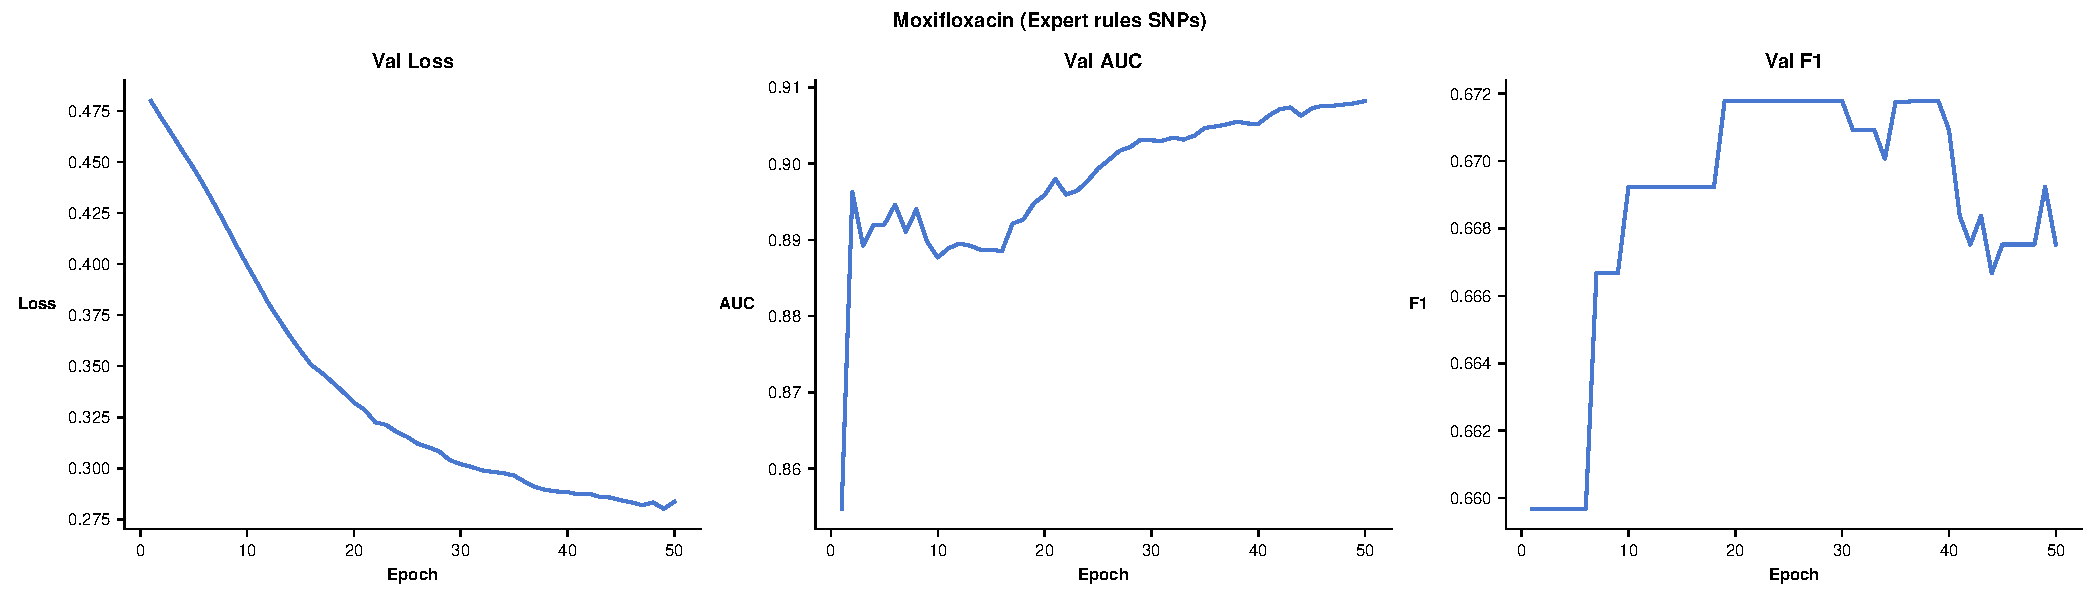
\includegraphics[width=\textwidth]{figures/expert_rules_moxifloxacin_learning_curves.pdf}
    \end{subfigure}
    \begin{subfigure}{\textwidth}
        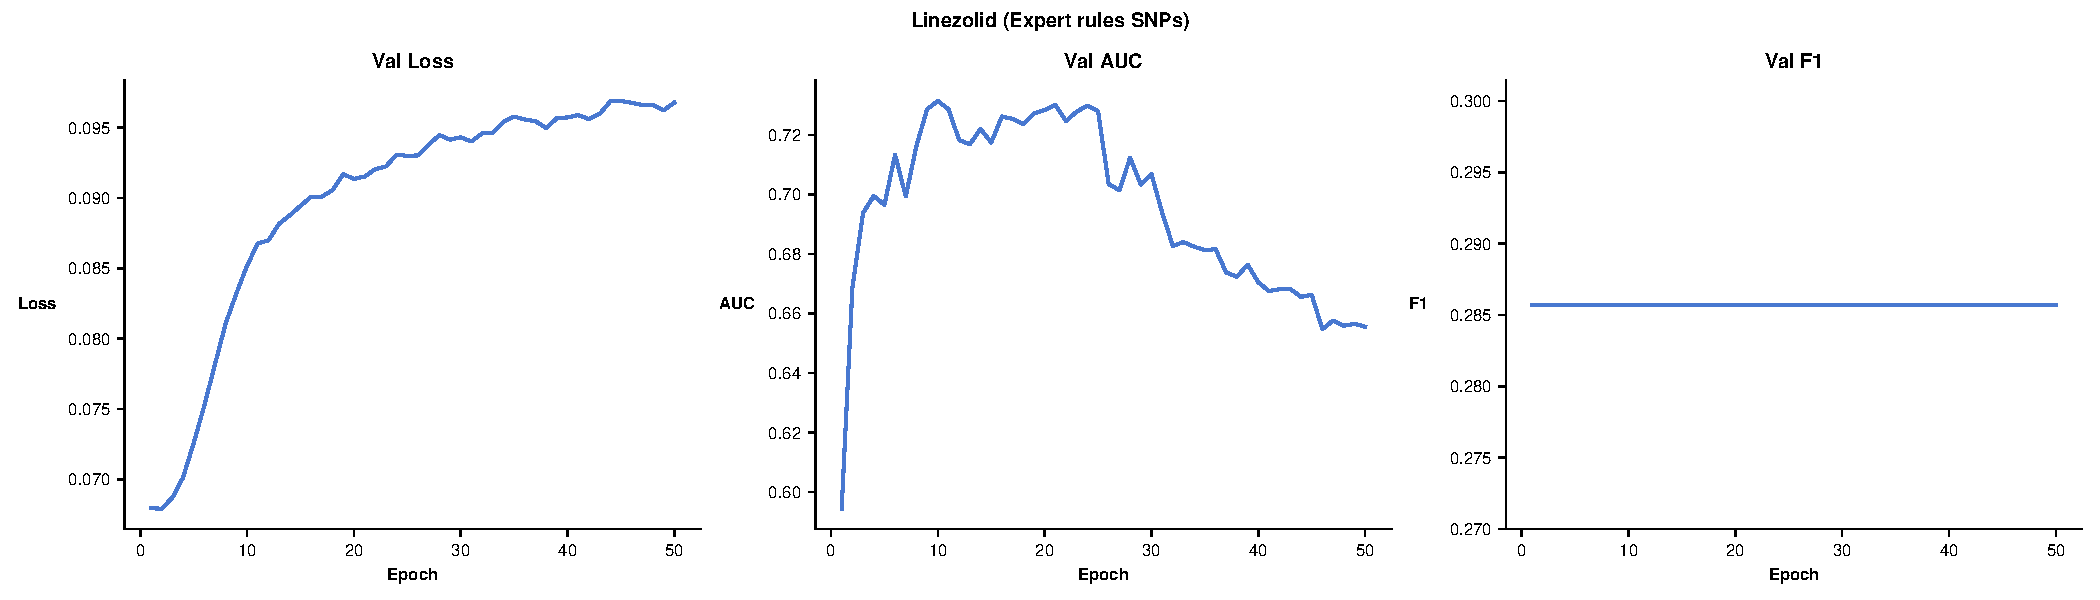
\includegraphics[width=\textwidth]{figures/expert_rules_linezolid_learning_curves.pdf}
    \end{subfigure}
    \caption{Model performance across all drugs}  % caption only on last block
    \label{fig:all_drugs}
\end{figure}

\input{chapters/filtlr}


\subsection{Feature Ablation and SNP Refinement}
\subsubsection{Drugs with reduced sensitivity post-ablation}
\begin{figure}[H]
    \centering
    \begin{subfigure}{0.45\textwidth}
        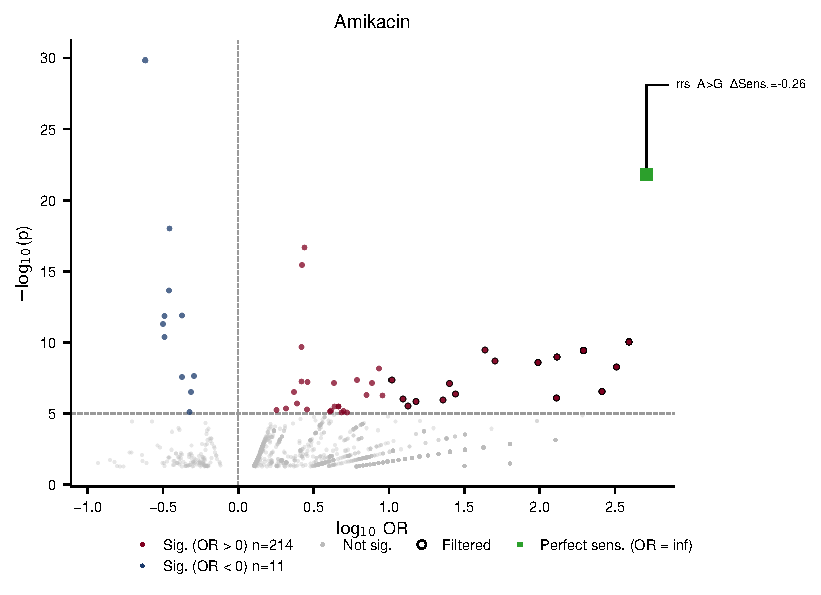
\includegraphics[width=\textwidth]{figures/plots/amikacin_volcano.pdf}
    \end{subfigure}
    \hfill
    \begin{subfigure}{0.45\textwidth}
        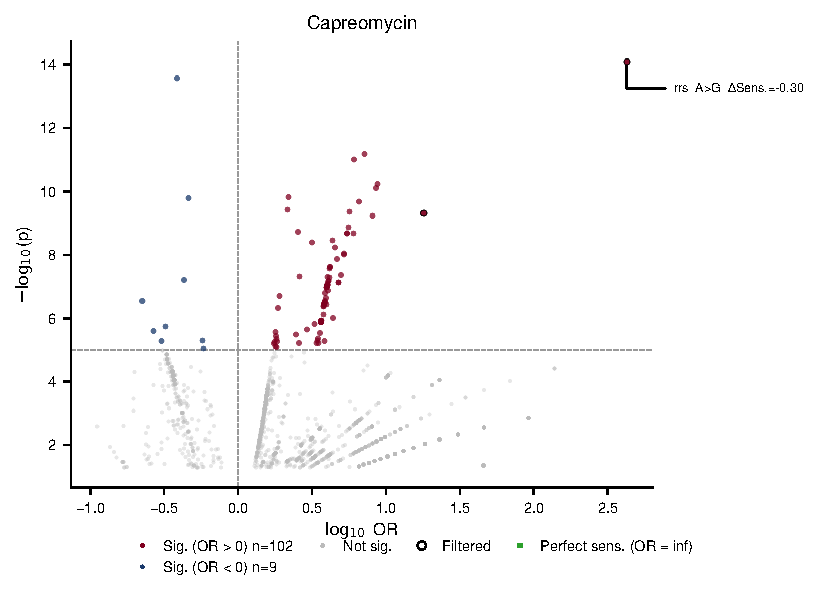
\includegraphics[width=\textwidth]{figures/plots/capreomycin_volcano.pdf}
    \end{subfigure}
    \hfill
    \begin{subfigure}{0.45\textwidth}
        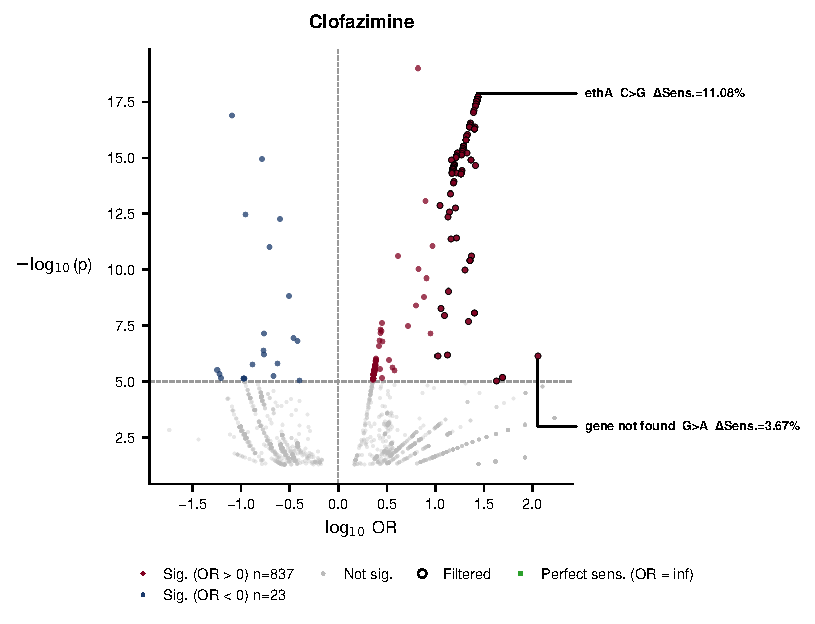
\includegraphics[width=\textwidth]{figures/plots/clofazimine_volcano.pdf}
    \end{subfigure}
    \hfill
    \begin{subfigure}{0.45\textwidth}
        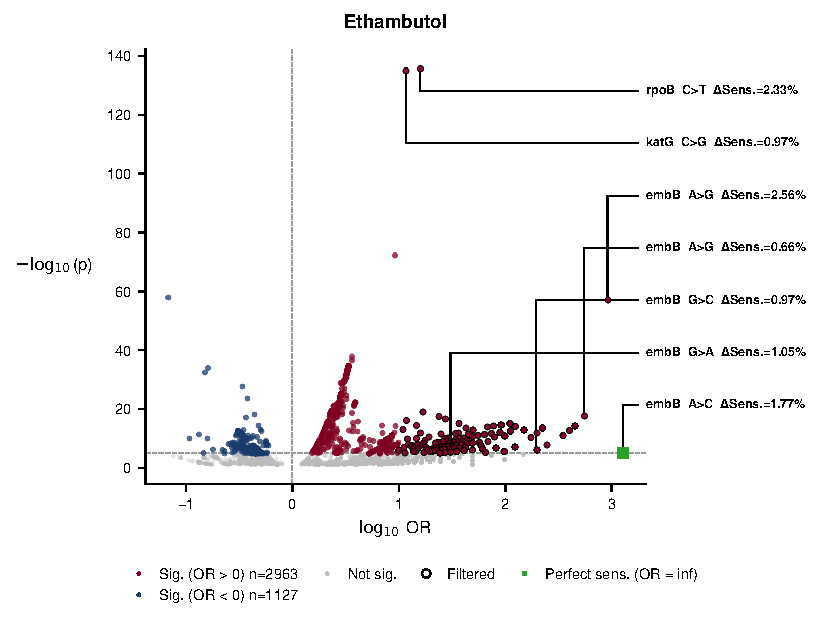
\includegraphics[width=\textwidth]{figures/plots/ethambutol_volcano.pdf}
    \end{subfigure}
    \hfill
    \begin{subfigure}{0.45\textwidth}
        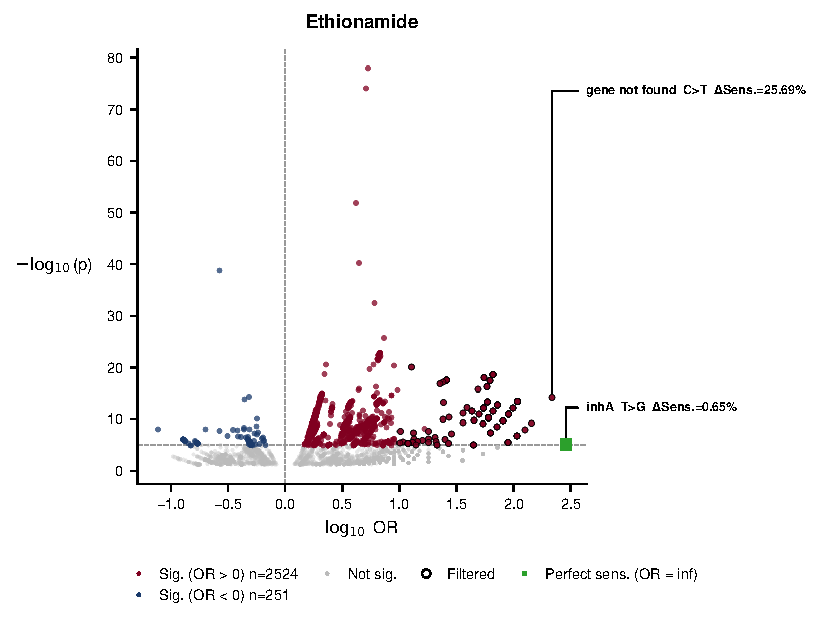
\includegraphics[width=\textwidth]{figures/plots/ethionamide_volcano.pdf}
    \end{subfigure}
     \hfill
    \begin{subfigure}{0.45\textwidth}
        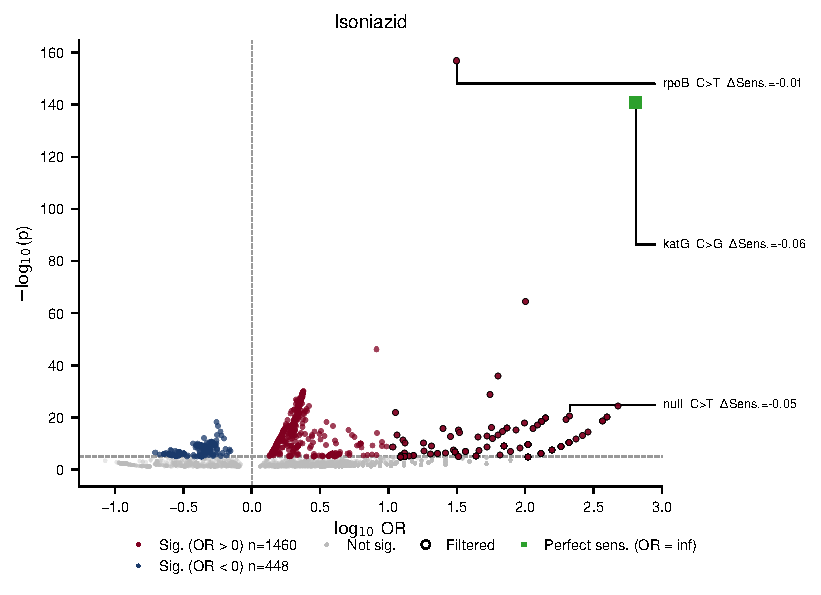
\includegraphics[width=\textwidth]{figures/plots/isoniazid_volcano.pdf}
    \end{subfigure}
    \hfill
    \begin{subfigure}{0.45\textwidth}
        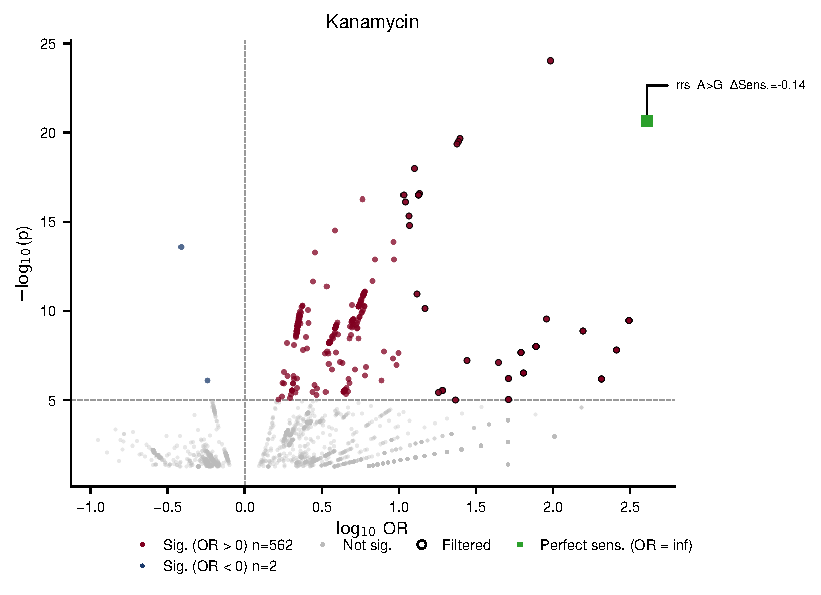
\includegraphics[width=\textwidth]{figures/plots/kanamycin_volcano.pdf}
    \end{subfigure}

\end{figure}

\begin{figure}
  \continuedfloat
  \begin{subfigure}{0.45\textwidth}
      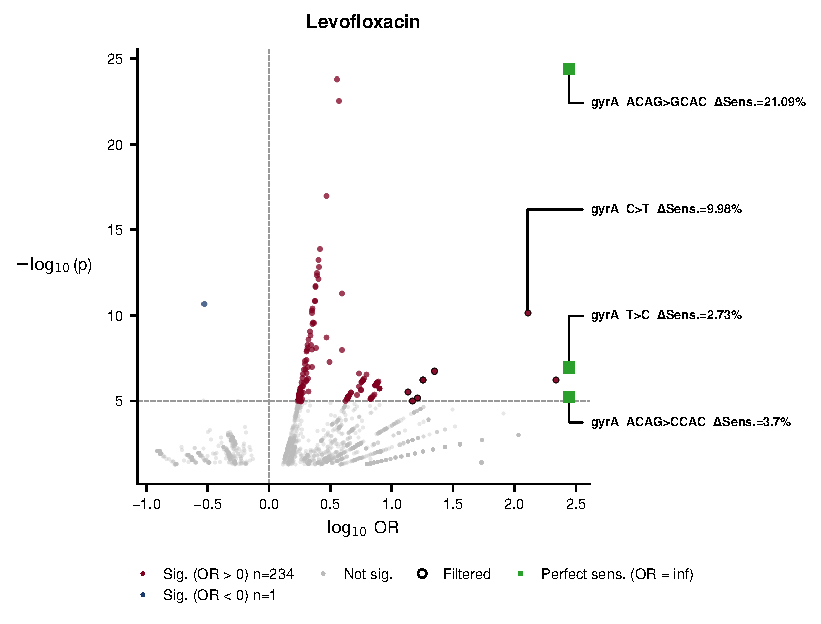
\includegraphics[width=\textwidth]{figures/plots/levofloxacin_volcano.pdf}
  \end{subfigure}
    \hfill
  \begin{subfigure}{0.45\textwidth}
      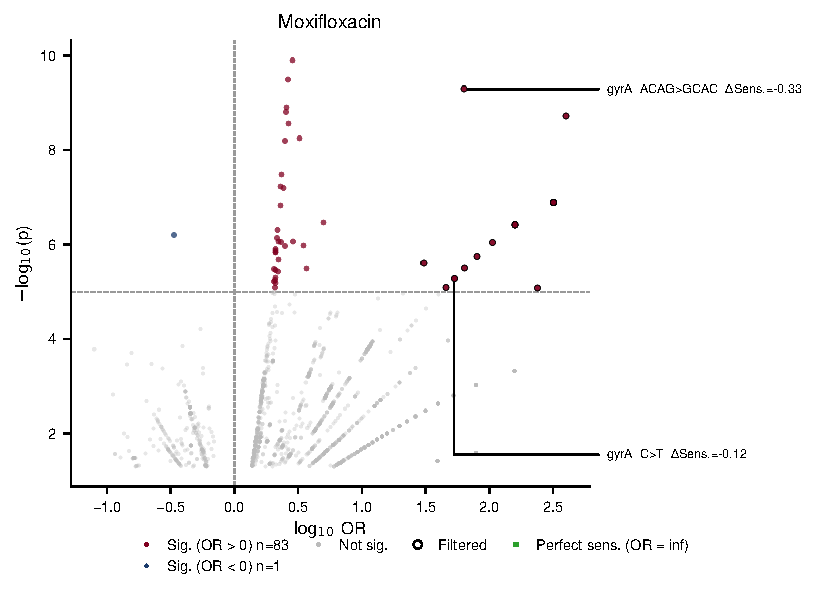
\includegraphics[width=\textwidth]{figures/plots/moxifloxacin_volcano.pdf}
  \end{subfigure}
    \hfill
  \begin{subfigure}{0.45\textwidth}
      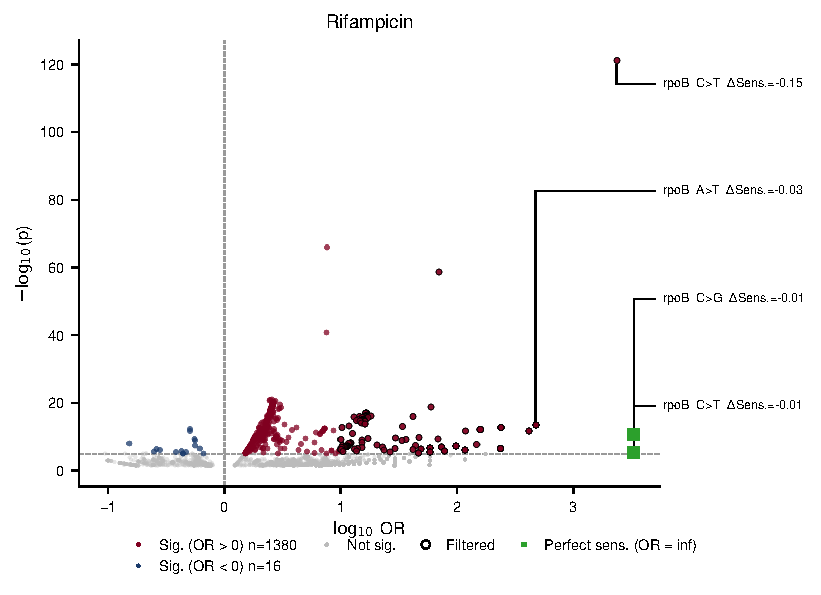
\includegraphics[width=\textwidth]{figures/plots/rifampicin_volcano.pdf}
  \end{subfigure}
    \hfill
  \begin{subfigure}{0.45\textwidth}
      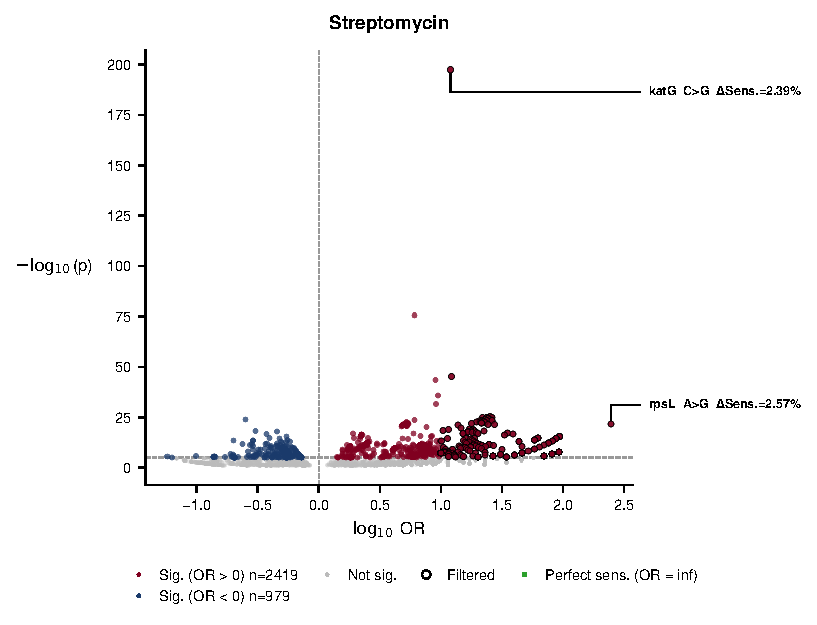
\includegraphics[width=\textwidth]{figures/plots/streptomycin_volcano.pdf}
  \end{subfigure}
\end{figure}

\subsubsection{Drugs with no change post-ablation}
\begin{figure}[H]
    \centering
    \begin{subfigure}{0.45\textwidth}
        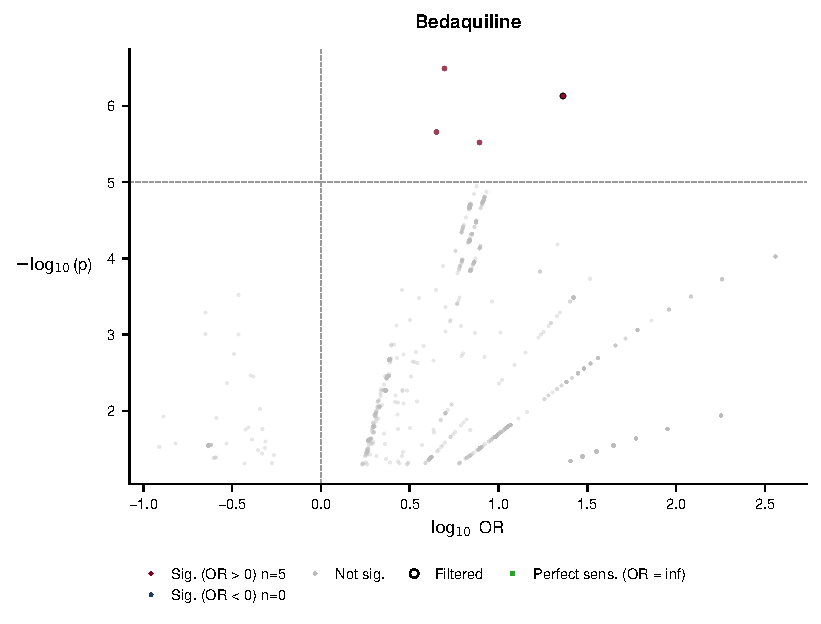
\includegraphics[width=\textwidth]{figures/plots/bedaquiline_volcano.pdf}
    \end{subfigure}
    \hfill
    \begin{subfigure}{0.45\textwidth}
        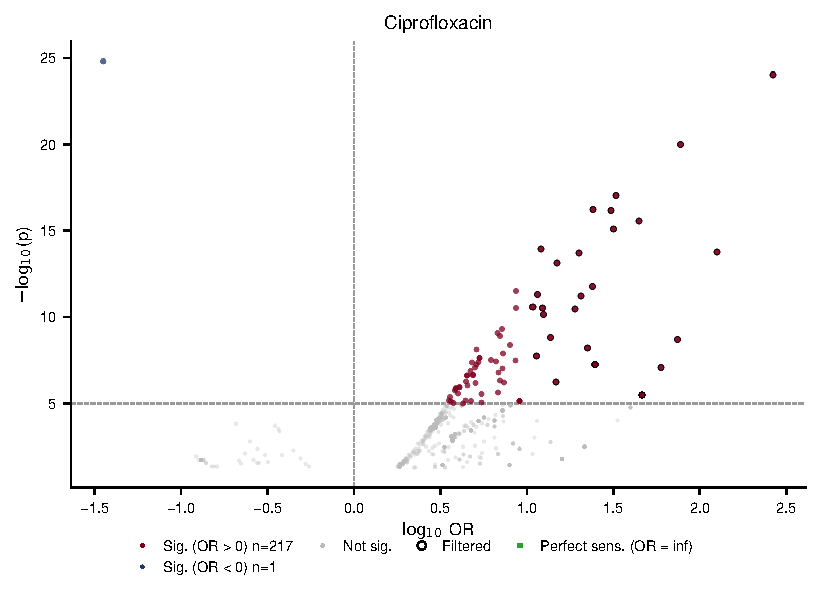
\includegraphics[width=\textwidth]{figures/plots/ciprofloxacin_volcano.pdf}
    \end{subfigure}
    \hfill
    \begin{subfigure}{0.45\textwidth}
        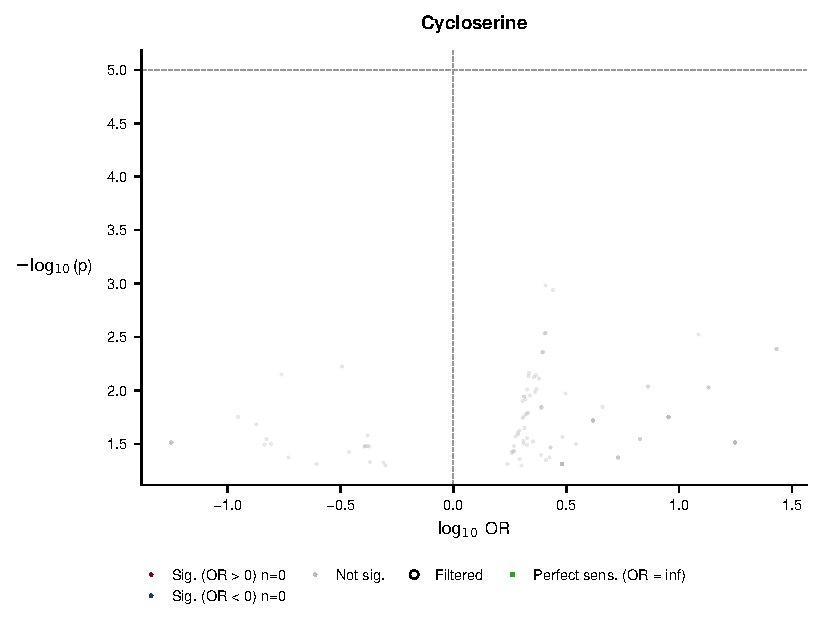
\includegraphics[width=\textwidth]{figures/plots/cycloserine_volcano.pdf}
    \end{subfigure}
    \hfill
    \begin{subfigure}{0.45\textwidth}
        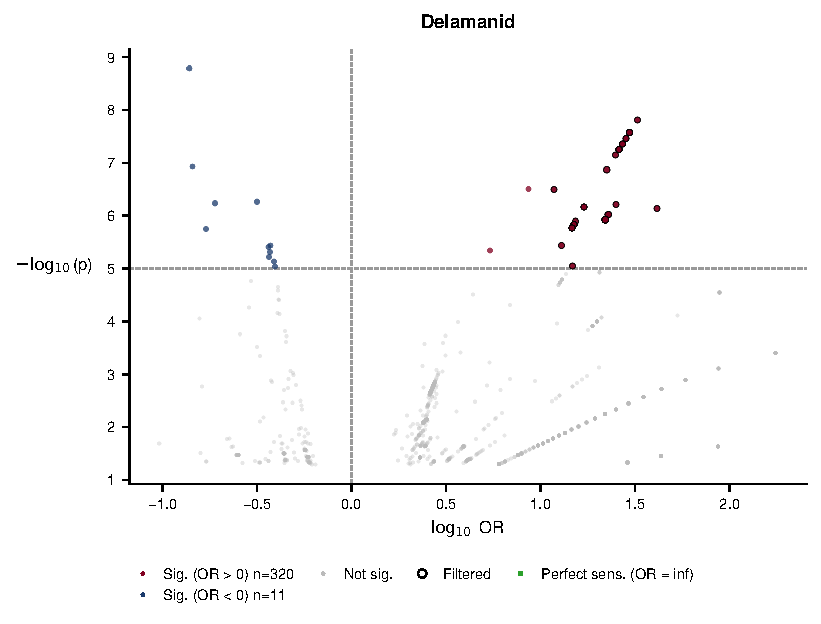
\includegraphics[width=\textwidth]{figures/plots/delamanid_volcano.pdf}
    \end{subfigure}
    \hfill
    \begin{subfigure}{0.45\textwidth}
        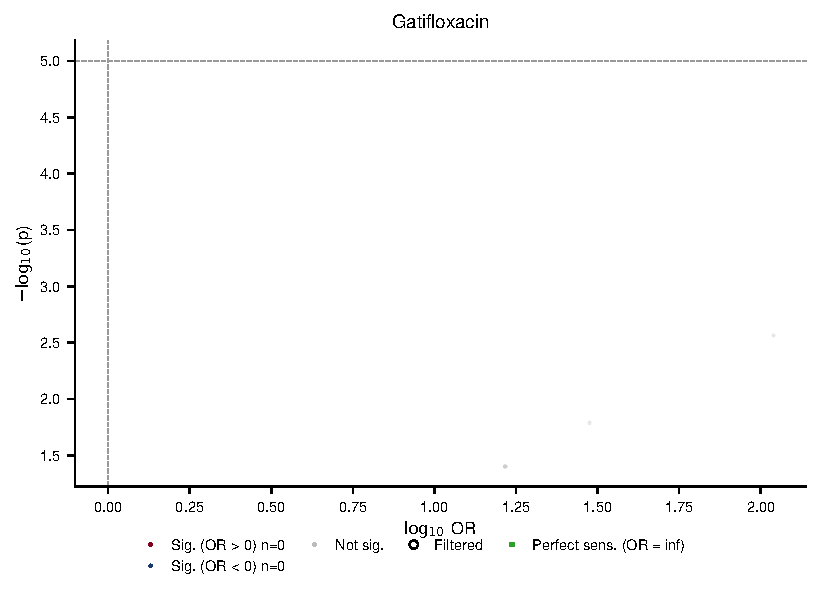
\includegraphics[width=\textwidth]{figures/plots/gatifloxacin_volcano.pdf}
    \end{subfigure}

\end{figure}

\begin{figure}[H]
  \continuedfloat
  \begin{subfigure}{0.45\textwidth}
      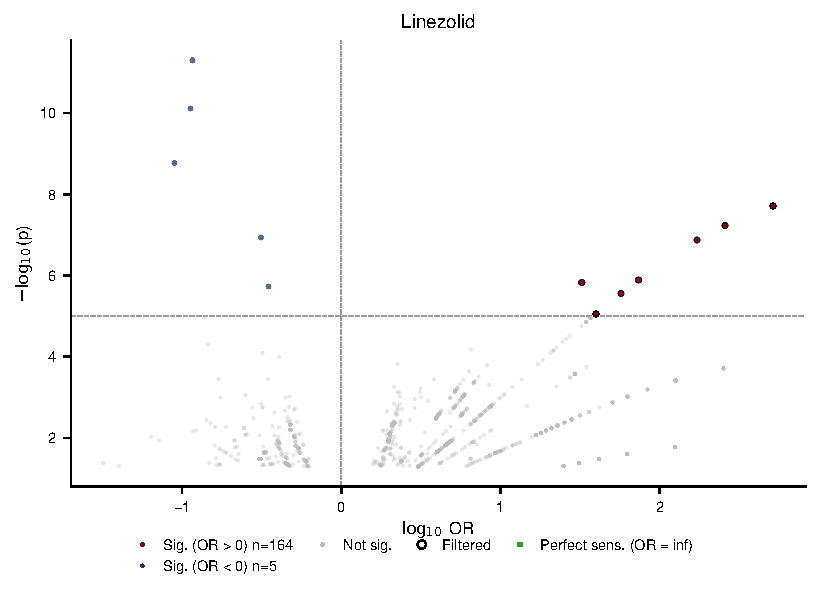
\includegraphics[width=\textwidth]{figures/plots/linezolid_volcano.pdf}
  \end{subfigure}
    \hfill
  \begin{subfigure}{0.45\textwidth}
      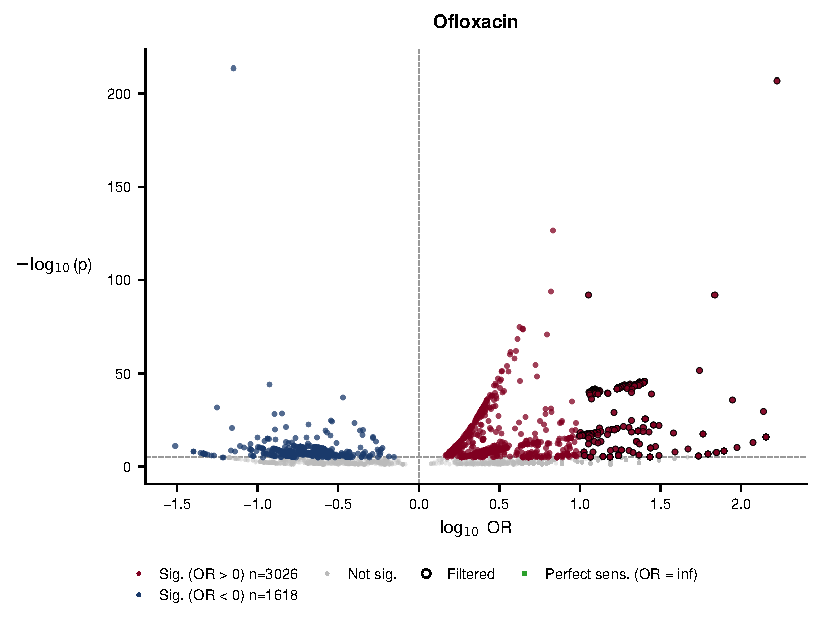
\includegraphics[width=\textwidth]{figures/plots/ofloxacin_volcano.pdf}
  \end{subfigure}
    \hfill
  \begin{subfigure}{0.45\textwidth}
      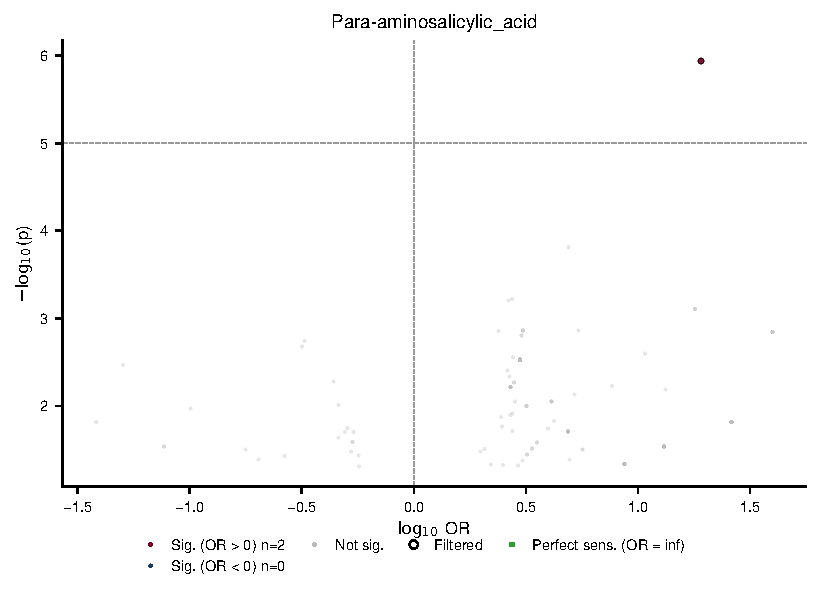
\includegraphics[width=\textwidth]{figures/plots/para-aminosalicylic_acid_volcano.pdf}
  \end{subfigure}
    \hfill
  \begin{subfigure}{0.45\textwidth}
      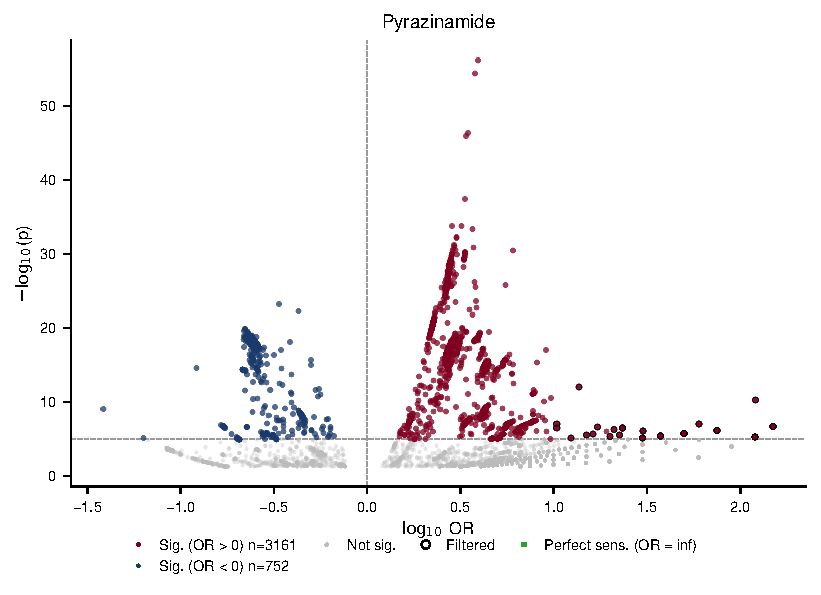
\includegraphics[width=\textwidth]{figures/plots/pyrazinamide_volcano.pdf}
  \end{subfigure}
    \hfill
  \begin{subfigure}{0.45\textwidth}
      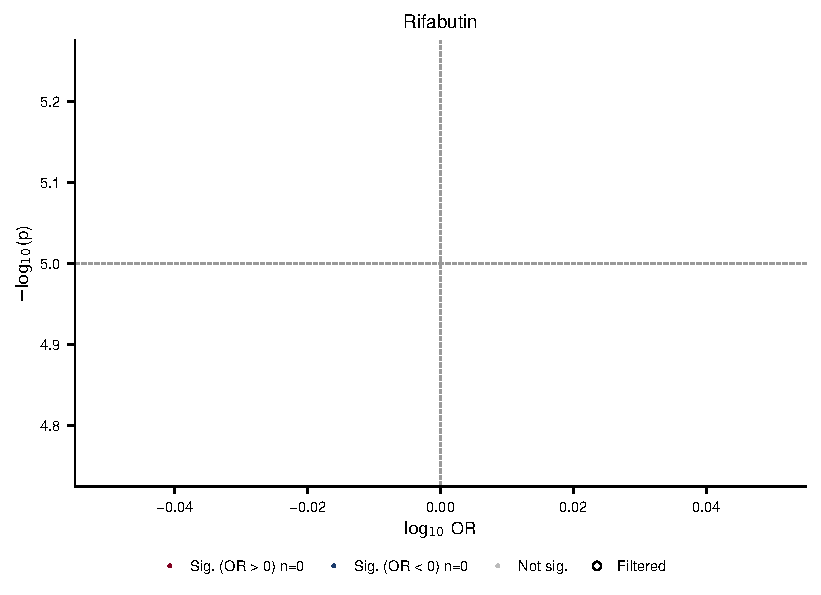
\includegraphics[width=\textwidth]{figures/plots/rifabutin_volcano.pdf}
  \end{subfigure}
    \hfill
  \begin{subfigure}{0.45\textwidth}
      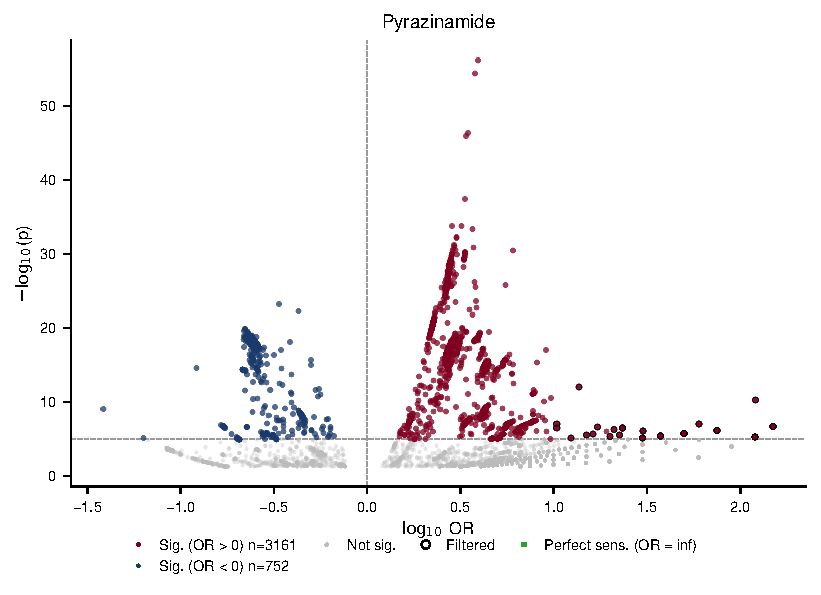
\includegraphics[width=\textwidth]{figures/plots/pyrazinamide_volcano.pdf}
  \end{subfigure}
\end{figure}



